% Created 2019-10-28 Mon 11:45
% Intended LaTeX compiler: pdflatex
\documentclass[11pt]{article}
\usepackage[utf8]{inputenc}
\usepackage{lmodern}
\usepackage[T1]{fontenc}
\usepackage{fixltx2e}
\usepackage{graphicx}
\usepackage{longtable}
\usepackage{float}
\usepackage{wrapfig}
\usepackage{rotating}
\usepackage[normalem]{ulem}
\usepackage{amsmath}
\usepackage{textcomp}
\usepackage{marvosym}
\usepackage{wasysym}
\usepackage{amssymb}
\usepackage{amsmath}
\usepackage[theorems, skins]{tcolorbox}
\usepackage[version=3]{mhchem}
\usepackage[numbers,super,sort&compress]{natbib}
\usepackage{natmove}
\usepackage{url}
\usepackage{minted}
\usepackage{underscore}
\usepackage[linktocpage,pdfstartview=FitH,colorlinks,
linkcolor=blue,anchorcolor=blue,
citecolor=blue,filecolor=blue,menucolor=blue,urlcolor=blue]{hyperref}
\usepackage{attachfile}
\usepackage[left=1in, right=1in, top=1in, bottom=1in, nohead]{geometry}
\geometry{letterpaper}
\usepackage{outline}
\usepackage{amsmath}
\usepackage{graphicx}
\usepackage{epstopdf}
\usepackage{siunitx}
\usepackage{bm}
\usepackage{framed,color}
\definecolor{shadecolor}{rgb}{1.0,0.8,0.3}
\usepackage{parskip}
\usepackage[version=3]{mhchem}
\usepackage[labelfont=bf]{caption}
\usepackage{hyperref}
\hypersetup{colorlinks=true,urlcolor=blue}
\setlength{\headheight}{15.2pt}
\usepackage{fancyhdr}
\pagestyle{fancy}
\fancyhf{}
\renewcommand{\headrulewidth}{0.5pt}
\renewcommand{\footrulewidth}{0.5pt}
\lfoot{\today}
\cfoot{\copyright\ 2019 W.\ F.\ Schneider}
\rfoot{\thepage}
\lhead{\em{Computational Chemistry}}
\rhead{ND CBE 60547}
\def\dbar{{\mathchar'26\mkern-12mu d}}
\setcounter{secnumdepth}{3}
\author{William F. Schneider}
\date{\today}
\title{Lecture Notes for CBE 60547}
\begin{document}

\setcounter{tocdepth}{1}
\tableofcontents

\begin{OPTIONS}
\end{OPTIONS}

\section{Introduction}
\label{sec:org610a55b}
\subsection{What do we care about?}
\label{sec:orgf465298}

Things chemistry/materials-related:

\begin{itemize}
\item What are the properties of atoms?
\item What molecules do they make?  What other substances do they make?
\item What are the shapes of those molecules?  Structures of those solids?  Properties of them?
\item How do those substances react with each other?
\item What are the energies of those reactions?
\item What are the rates of those reactions?
\item What is the strongest substance?
\item How do we make a substance to do\ldots{}.?
\item add your own questions\ldots{}.
\end{itemize}

Things that relate to the \emph{chemical} properties of substances.

\subsection{How are we going to figure these out?  With only a computer?}
\label{sec:orgad2fd13}
\begin{description}
\item[{1926}] Erwin Schr\"{o}dinger equation: \(\hat{H}\Psi=E\Psi\)
\item[{1929}] Paul Dirac, British physicist
\end{description}

\begin{quote}
The fundamental laws necessary for the mathematical treatment of a
large part of physics and the whole of chemistry are thus \emph{completely
known}, and the difficulty lies only in the fact that application of
these laws leads to equations that are \emph{too complex to be solved}.

It therefore becomes desirable that \emph{approximate practical methods} of
applying quantum mechanics should be developed, which can lead to an
explanation of the main features of complex atomic systems without
too much computation.
\end{quote}

\begin{description}
\item[{1930's-1950's}] Elaboration, analytical applications

\item[{1950's}] Computers start to appear for technical applications

\item[{1960's}] Density functional theory emerges.

\item[{1960's-1970's}] Numerical solutions of Schr\"{o}dinger equation for atoms/molecules---expert users

\item[{1980's}] ``Supercomputer'' era---routine use of computational chemistry software becomes possible
\end{description}
\begin{figure}[htbp]
\centering
\includegraphics[width=0.2\textwidth]{./Images/CrayYMPb.jpg}
\caption{Ohio State Cray Y-MP supercomputer, ca. 1989.  World's fastest computer at the time.  333 MFlop top speed, 512 Mb RAM}
\end{figure}

\begin{description}
\item[{1990's}] ``Chemical accuracy'' era---very precise solutions routinely available, for a cost!  See \href{./Resources/1994\_WFS\_JPC.pdf}{Schneider, \emph{JPC} \textbf{1994}}.

\item[{1990's}] Density functional theory (DFT) allows applications to solids/surfaces/liquids to become common. See \href{./Resources/1998\_Hass\_Science.pdf}{Hass, \emph{Science}, \textbf{1998}}

\item[{1990's}] Visualization moves to the desktop

\item[{2000's}] Computational ``screening,'' materials discovery (\href{http://www.crc.nd.edu/\~wschnei1/courses/CBE\_547/Resources/2010\_Gurkan\_JPCL.pdf}{Gurkan, \emph{J. Phys. Chem. Lett.}, \textbf{2010}}), materials genome (\url{https://materialsproject.org/}).

\item[{Today}] Computational chemistry widely integrated into all aspects of chemical, materials, biological research
\end{description}

\texttt{Computational chemistry} is now so vast it is impossible to cover everything completely.  We limit ourselves to quantum-mechanics-based calculations.

\subsection{Our goals}
\label{sec:orgd5865cb}
\begin{enumerate}
\item Understand when it is appropriate to use quantum-mechanics methods.
\item Be able to state the basic theoretical, mathematical, and numerical concepts behind quantum mechanical ``wavefunction theory'' (WFT) and ``density functional theory,'' (DFT) calculations.
\item Understand the terminology and practical issues associated with doing quantum chemical simulations.
\item Get hands-on experience with these concepts using popular computational tools of today, including GAMESS for molecular systems and Vasp for condensed phase systems.
\item Learn how to set up, execute, and analyze results in a modern, Python notebook environment.
\item Learn how to apply the results of quantum chemical simulations to calculate things you care about.
\item Demonstrate an ability to formulate a problem and apply QM  methods to it.
\item Develop the skills to understand a literature paper in the area.
\end{enumerate}

\subsection{Reading resources}
\label{sec:org9554a72}
\begin{itemize}
\item These notes
\item Chris Cramer, \emph{Essentials of Computational Chemistry}, Wiley, 2004
\item Martin, \emph{Electronic Structure}, Cambridge, 2004
\item Sholl and Steckel, \emph{Density Functional Theory: A Practical Introduction}, Wiley, 2009
\item Kitchin book, \url{http://kitchingroup.cheme.cmu.edu/dft-book/}
\end{itemize}

\subsection{Software tools}
\label{sec:org825cd78}
\subsubsection{Notebooks}
\label{sec:org4a560f2}
\begin{itemize}
\item \href{https://jupyter.org/}{jupyter}/ipython
\item \href{https://www.gnu.org/software/emacs/}{emacs}/org-mode
\end{itemize}

\subsubsection{Molecular methods}
\label{sec:org785ec60}
\begin{itemize}
\item Avogadro environment \url{http://avogadro.cc/wiki/Main\_Page}
\item GAMESS code \url{http://www.msg.ameslab.gov/GAMESS/GAMESS.html}
\end{itemize}

\subsubsection{Supercell methods}
\label{sec:orgb94ee19}
\begin{itemize}
\item Vasp code \url{http://www.vasp.at/}
\item ASE environment \url{https://wiki.fysik.dtu.dk/ase/}
\end{itemize}

\subsubsection{Great for getting started}
\label{sec:orgc4a8472}
\begin{itemize}
\item Webmo \url{http://www.webmo.net/}
\end{itemize}
\newpage

\section{Refresher on Quantum Mechanics}
\label{sec:org038fc65}
\subsection{Why quantum mechanics?}
\label{sec:org519ae13}
Want to describe ``mechanics'' (equations of motion) of atomic-scale things, like electrons in atoms and molecules

Why? These ultimately determine the energy, the shape, and all the properties of matter.

\emph{de Broglie wavelength} (1924)
\begin{equation}
\lambda  = h/p = h/mv
\end{equation}
\begin{equation}
h  = \SI{6.626e-34}{J.s} \text{(Planck's constant)}
\end{equation}

\begin{center}
\begin{tabular}{lll}
\hline
 & Car & Electron\\
\hline
mass \(m\) & \SI{1000}{kg} & \SI{9.1e-31}{kg}\\
velocity \(v\) & \SI{100}{km/hr} & \SI{0.01}{c}\\
 & typical value on the highway & typical value in an atom\\
momentum \(p\) & \SI{2.8e-4}{kg.m/s} & \SI{2.7e-24}{kg.m/s}\\
wavelength \(\lambda\) & \SI{2.4e-38}{m} & \SI{2.4e-10}{m}\\
 & too small to detect.  Classical! & Comparable to size of an atom.\\
 &  & \emph{Must} treat with QM!\\
\hline
\end{tabular}
\end{center}

How to describe wave properties of an electron?  Schr\"{o}dinger equation (1926)

\begin{center}
Kinetic energy + Potential energy = Total Energy
\end{center}

Expressed as differential equation (Single particle, non-relativistic):
\begin{equation}
-\frac{\hbar^2}{2m}\nabla^2 \Psi(\mathbf{r},t) + V(\mathbf{r},t)  \Psi(\mathbf{r},t) = -i \hbar \frac{\partial}{\partial t}  \Psi(\mathbf{r},t)
\end{equation}

If the potential \(V\) is time-invariant, can use separation of variables to
show that the steady-state, time-independent solutions are characterized by an
energy \(E\) and described by:
\begin{eqnarray}
-\frac{\hbar^2}{2m}\nabla^2 \psi(\mathbf{r}) + V(\mathbf{r})  \psi(\mathbf{r}) = E \psi(\mathbf{r}) \\
\Psi(\mathbf{r},t) = \psi(\mathbf{r})e^{-iEt/\hbar}
\end{eqnarray}

\subsection{Postulates of non-relativistic quantum mechanics}
\label{sec:org303b511}
\begin{table} 
\begin{center}
    \caption{\large{Postulates of Non-relativistic Quantum Mechanics}}
   \begin{description}
    \item[Postulate 1:] {{\bf The physical state of a system is completely described by
        its wavefunction $\Psi$.}  In general, $\Psi$ is a complex function of the spatial
      coordinates and time.  $\Psi$ is required to be:}
    \begin{outline}
      \item{Single-valued}
      \item {continuous and twice differentiable}
      \item {square-integrable ($\int \Psi^*\Psi d\tau$ is defined over all finite domains)}
      \item {For bound systems, $\Psi$ can always be normalized such that $\int \Psi^*\Psi d\tau=1$}
    \end{outline}

  \item[Postulate 2:]  To every physical observable quantity $M$ there corresponds a
    Hermitian operator $\hat{M}$.  {\bf The only observable values of $M$ are the
      eignevalues of $\hat{M}$.}
    \begin{center}
    \begin{tabular}[h]{ccc}
      \hline
{\bf Physical quantity} & {\bf Operator} & {\bf Expression} \\
\hline
Position $x,y,z$ & $\hat{x},\hat{y},\hat{z}$ & $x\cdot, y\cdot, z\cdot$ \\ \\
Linear momentum $p_x, \ldots$ & $\hat{p}_x,\ldots $ & $\displaystyle -i\hbar\frac{\partial}{\partial
  x},\ldots $\\
Angular momentum $l_x, \ldots$ & $\hat{p}_x,\ldots $ & $\displaystyle -i\hbar \left
  (y\frac{\partial}{\partial z}-z\frac{\partial}{\partial y}\right ), \ldots $ \\
Kinetic energy $T$ & $\hat{T}$ & $\displaystyle -\frac{\hbar^2}{2m}\nabla^2$ \\
Potential energy $V$ & $\hat{V}$ & $V({\bf r},t)$ \\
Total energy $E$ & $\hat{H}$ & $\displaystyle -\frac{\hbar^2}{2m}\nabla^2+V({\bf r},t)$\\ \\
\hline
    \end{tabular}
  \end{center}
    \item[Postulate 3:] {If a particular observable $M$ is measured many times on many
      identical systems is a state $\Psi$, the average resuts with be the expectation
      value of the operator $\hat{M}$:
      \begin{equation*}
        \langle M \rangle = \int \Psi^* (\hat{M}\Psi)d{\bf\tau}
      \end{equation*}}
    \item[Postulate 4:] {The energy-invariant states of a system are solutions of the equation
        \begin{eqnarray*}
          \hat{H}\Psi({\bf r},t) & = & i\hbar\frac{\partial}{\partial t}\Psi({\bf r},t) \\
          \hat{H} & = & \hat{T}+\hat{V}
        \end{eqnarray*}
      The time-independent, stationary states of the system are solutions to the equation
      \begin{equation*}
        \hat{H}\Psi({\bf r}) = E\Psi(\bf{r})
      \end{equation*}
}
    \item[Postulate 5:] (The {\bf uncertainty principle}.)  Operators that do not commute
      $(\hat{A}(\hat{B}\Psi)\neq\hat{B}(\hat{A}\Psi))$ are called {\em conjugate}.
      Conjugate observables cannot be determined simultaneously to arbitrary accuracy.
      For example, the standard deviation in the measured positions and momenta of
      particles all described by the same $\Psi$ must satisfy $\Delta x\Delta p_x \geq \hbar/2$.
    \end{description}
\end{center}
\end{table}

\subsection{Notes on constants and units}
\label{sec:orgd60dd15}
Resource on physical constants: \url{http://physics.nist.gov/cuu/Constants/}
Resource for unit conversions: \url{http://www.digitaldutch.com/unitconverter/}

Unit converter available in Calc mode in \href{https://www.gnu.org/software/emacs/}{Gnu emacs} \textbf{highly recommended}

\begin{table}[htbp]
\caption{Atomic units common for quantum mechanical calculations (see \url{http://en.wikipedia.org/wiki/Atomic\_units})}
\centering
\begin{tabular}{llll}
\hline
 & Atomic unit & SI unit & Common unit\\
\hline
Charge & \(e = 1\) & \SI{1.6021e-19}{C} & \\
Length & \(a_0 = 1\) (bohr) & \SI{5.29177e-11}{m} & \SI{0.529177}{\AA}\\
Mass & \(m_e = 1\) & \SI{9.10938e-31}{kg} & \\
Angular momentum & \(\hbar = 1\) & \SI{1.054572e-34}{J.s} & \\
Energy & \(E_h = 1\) (hartree) & \SI{4.359744e-18}{J} & \SI{27.2114}{eV}\\
Electrostatic force & \(1/(4\pi\epsilon_0) = 1\) & \SI{8.987552e-9}{N.m^2/C^2} & \\
Boltzmann constant &  & \SI{1.38065e-23}{J\per K} & \SI{8.61733e-5}{eV/K}\\
\hline
\end{tabular}
\end{table}


\begin{center}
Energy units
1 eV = \SI{1.60218e-19}{J} = \SI{96.485}{kJ/mol} = \SI{8065.5}\{cm\(^{\text{-1}}\)\} = \SI{11064}{K.k_B}
\end{center}

\subsection{Example: Energy states of a particle in a box}
\label{sec:org933ed2d}

System defined by potential experienced by particle:

\(V(\mathbf{r}) = 0,\qquad 0 < x,y,z < L\)

\(V(\mathbf{r}) = \infty,\qquad x,y,z \leq 0,\ x,y,z \geq L\)

\begin{center}
\begin{center}
\includegraphics[width=0.3\textwidth]{./Images/Cube.png}
\end{center}
\end{center}

3D box \(\rightarrow\) 3 degrees of freedom/coordinates

\textbf{Schr\"{o}dinger equation}
\begin{equation}
-\frac{\hbar^2}{2m_e} \left ( \frac{\partial^2 }{\partial x^2} + \frac{\partial^2 }{\partial y^2} + \frac{\partial^2 }{\partial z^2} \right ) \psi(x,y,z) = E \psi(x,y,z)
\end{equation}
\begin{equation}
\psi(x,y,z) = 0, \quad x,y,z \leq 0,\ x,y,z \geq L
\end{equation}

A second-order, linear, partial differential equation.  Boundary value problem. Solve by separation of variables.  Postulate \(\psi(x,y,z) = X(x)Y(y)Z(z)\). Substituting and rearrange to get

\begin{equation}
-\frac{\hbar^2}{2m_e} \left (\frac{1}{X(x)}\frac{\partial^2 X(x)}{\partial x^2} + \frac{1}{Y(y)}\frac{\partial^2 Y(y)}{\partial y^2} + \frac{1}{Z(z)}\frac{\partial^2 Z(z)}{\partial z^2} \right ) = E \qquad 0 < x,y,z <L
\end{equation}

ftn x + ftn y + ftn z = constant \(\rightarrow\) each term must be constant.

\textbf{Equation for each dimension}
\begin{equation}
-\frac{\hbar^2}{2m_e}\frac{\partial^2 X(x)}{\partial x^2} = E_x X(x), \qquad X(0)=X(L) = 0
\end{equation}

Seek function that twice differentiated returns itself and satisfies boundary conditions.
\begin{equation}
X(x) = \sin\frac{n_x\pi x}{L},\qquad n_x = 1,2,3,\ldots
\end{equation}

\begin{equation}
E_{n_x} = \frac{n_x^2\pi^2\hbar^2}{2 m_e L^2}
\end{equation}

Solutions called \emph{eigenfunctions} (or \emph{wavefunctions}) and \emph{eigenvalues}.  Characterized
by \emph{quantum numbers}, one for each degree of freedom.  These (and all QM) solutions have
certain special properties, including that they \emph{orthonormal} and form a \emph{complete set}.

\textbf{Normalization}

Seek a constant such that the inner eigenfunction product is unity.
\begin{eqnarray}
C^2 \int_0^L \sin^2 \frac{n_x\pi x}{L} dx = C^2 L/2 = 1 \rightarrow C=\pm\sqrt{\frac{2}{L}}\\
X(x) = \pm\sqrt{\frac{2}{L}}\sin\frac{n_x\pi x}{L},\qquad n_x = 1,2,3,\ldots
\end{eqnarray}

\textbf{Orthonormal}
\begin{equation}
\langle X_{n_x} | X_{n^\prime_x} \rangle = \delta_{n_{x},n_x^\prime}\qquad
\text{Dirac notation}
\end{equation}

\begin{center}
\includegraphics[width=0.75\textwidth]{./Images/1DPIAB.png}
\end{center}

\begin{itemize}
\item Energy increase with number of \emph{nodes}.

\item Is this real?  See \href{http://dx.doi.org/10.1021/jp053496l}{Ho, \emph{J. Phys. Chem. B} \textbf{2005}, \emph{109}, 20657}.  Where \emph{is} the electron?
\end{itemize}

\textbf{Complete set}
Any function on the same domain that satisfies the same boundary conditions can be represented as a linear combination of these solutions:
\begin{eqnarray}
f(x) &=& \sum_i \left \{\int_0^L X_i(x) f(x) dx \right \}  X_i(x)  = \sum_i C_i X_i(x)\\
|f\rangle &= &\sum_i |X_i\rangle\langle X_i | f\rangle\quad\text{Dirac notation}
\end{eqnarray}
Illustrates idea of a basis set. These functions are the basis in ``plane wave'' supercell methods.

\textbf{Three-dimensional solutions}
\begin{equation}
\psi(x,y,z) = X(x)Y(y)Z(z) = \left ( \frac{2}{L} \right )^{3/2} \sin\frac{n_x\pi x}{L}\sin\frac{n_y\pi y}{L}\sin\frac{n_z\pi z}{L},\qquad n_{x},n_{y},n_{z}=1,2,3,\ldots
\end{equation}
\begin{equation}
\label{eq:2}
E = E_{x}+E_{y}+E_{z}=\frac{(n_{x}^{2}+n_{y}^{2}+n_{z}^{2}) \pi^{2}\hbar^{2}}{2 m L^{2}}
\end{equation}

\begin{center}
\includegraphics[width=0.5\textwidth]{./Images/2DSine1.png}
\end{center}
\begin{center}
\includegraphics[width=0.5\textwidth]{./Images/2DSine2.png}
\end{center}


\begin{figure}[htbp]
\centering
\includegraphics[width=.9\linewidth]{./Images/3DEnergyStates.png}
\caption{Energy sates of 3D Particle in a box}
\end{figure}

Properties of solutions:
\begin{itemize}
\item Symmetry of system introduces degeneracy in solutions
\item Energy depends on volume \(\rightarrow\) pressure!
\end{itemize}

\newpage

\section{Hydrogen atom: simplest chemical ``thing''}
\label{sec:org85a3986}
\subsection{Schr\"{o}dinger equation}
\label{sec:org08c21bf}
Place massive nucleus at origin and describe position of electron in spherical coordinates

\begin{center}
\includegraphics[width=0.3\textwidth]{./Images/spherical.png}
\end{center}

\begin{eqnarray}
\left\{-\frac{\hbar^2}{2m_e}\nabla^2 + V(r)\right\} \psi(\bm{r}) &=& E \psi(\bm{r})\\
V(r) &=& -\frac{e^2}{4\pi\epsilon_0}\frac{1}{|\bm{r}|}
\end{eqnarray}
Coulomb potential---our nemesis!  Decays slowly with distance.  Boundary conditions?
\begin{table}[]
   \begin{center}
   \caption{Hydrogen atom}
    \label{Hydrogen atom}
\begin{tabular}[h]{|c|}
\hline
 \\
$\displaystyle       V(r) = -\frac{e^2}{4\pi\epsilon_0}\frac{1}{r}, 0 < r< \infty$ \\
 \\
$\displaystyle     \hat H = -\frac{\hbar^2}{2m_e}\left \{ \frac{1}{r^2}\left [
  \frac{\partial}{\partial r}r^2\frac{\partial}{\partial r}  \right ] - \frac{\hat{L}^2}{\hbar^2 r^2} \right \} +V(r)$ \\
\\
$\displaystyle     \hat L^2 = -\hbar^2 \left [
  \frac{1}{\sin^2\theta}\frac{\partial^2}{\partial \phi^2}+\frac{1}{\sin
    \theta}\frac{\partial}{\partial \theta}\left ( \sin \theta
    \frac{\partial}{\partial \theta}\right ) \right ] $ \\
\\
$\displaystyle \psi(r,\theta,\phi) = R(r)Y_{l,m_l}(\theta,\phi) $ \\
\\
$\displaystyle   \left \{ -\frac{\hbar^2}{2m_e}
            \frac{d}{dr^2}  + \frac{\hbar^2
              l(l+1)}{2 m_e r^2}
          -\frac{e^2}{4\pi\epsilon_0}\frac{1}{r}\right \} r R(r) = E r R(r) $ \\
\\
$\displaystyle R_{nl}(r) = N_{nl} e^{-x/2} x^l L_{nl}(x),\ \ \  x = \frac{2 r}{n a_0} $
\\
$\displaystyle P_{nl}(r) = r^2 R_{nl}^2 $
\\
\\
$\displaystyle n = 1, 2, \ldots,\ \  l = 0, \ldots, n-1 \ \ m_l = 0,\pm 1, \ldots, \pm l$
\\
\\
$\displaystyle N_{nl} = \sqrt{\left ( \frac{2}{na_0}\right )^3 \frac{(n-l-1)!}{2n(n+l)!}}$
\\
\\
$\displaystyle L_{10} = L_{21} = L_{32} = \ldots =1 \quad L_{20} = 2 - x \quad L_{31} = 4-x$
\\
\\
\\
$\displaystyle     E_{n}=-\frac{1}{2}\frac{\hbar^2}{m_e a_0^2}\frac{1}{n^2} =-\frac{E_H}{2}\frac{1}{n^2}$ \\
 \\
$\displaystyle |L| = \hbar \sqrt{l(l+1)}, L_z = m_l \hbar $ \\
\\
$\displaystyle \langle r \rangle = \left \{ \frac{3}{2} n^2 - \frac{1}{2} l(l+1) \right \} \frac{a_0}{Z} $ \\
\\
%%     \includegraphics[scale=0.4]{Images/H_atom} \\       
\hline
\end{tabular}
 \end{center}
\end{table}

\subsection{Analytical solutions}
\label{sec:org41bfb5b}
\begin{enumerate}
\item Separate: \(\psi(r,\theta,\phi)=R(r)\Theta(\theta,\phi)\)
\item Angular equation \(\hat{L}^2\Theta(\theta,\phi) = E_L\Theta(\theta,\phi)\)
\begin{enumerate}
\item \(\Theta=Y_{lm_l}(\theta,\phi)\) are ``spherical harmonics'', describe angular motion
\item Azimuthal quantum number \(l=0,1,...,n-1\), correspond to \(s\), \(p\), \(d\), \ldots orbital sub-shells; angular ``shape,'' number of angular nodes, angular momentum of electron
\item Magnetic quantum number \(m_l=-l,-l+1,...,l\), \ldots orientation of orbital
\end{enumerate}
\item Radial equation
\[\left \{ -\frac{\hbar^2}{2m_e}
            \frac{d}{dr^2}  + \frac{\hbar^2
              l(l+1)}{2 m_e r^2}
          -\frac{e^2}{4\pi\epsilon_0}\frac{1}{r}\right \} r R(r) = E r R(r)\]
\end{enumerate}

Solutions are a polynomial * exponential decay.  Exponential part called a \emph{Slater} function.  Larger the exponent, faster the
      decay.  Degree of polynomial determined by principle quantum number \(n=1,2,\ldots\).

Energy expression, corresponds to our conventional H atom spectrum
     \[E_n = -\frac{1}{n^2}\left(\frac{e^2}{2 a_0}\right) = -\SI{13.6}{eV}\cdot\frac{1}{n^2},\qquad n = 1,2,\ldots \]

Questions: Ionization energy of an H atom?  \(1s\rightarrow 2s\) energy?  Thermal populations?

Integrate out angular components to get radial probability function \(P_{nl}(r)=r^2 R_{nl}^2(r)\)
    \[\langle r\rangle = \int r P_{nl}(r) dr = \left(\frac{3}{2}n^2-l(l+1)\right)a_0\]

Note darn electron doesn't want to stay in the Coulomb well!
   Wavefunction extends beyond the classical region defined by \(E_n =
   V(r_\text{classical})\).  This phenomenon is called \emph{tunneling}, is
   a purely quantum mechanical effect, is pervasive in chemistry,
   leading for instance to chemical bonding.


\begin{figure}[htbp]
\centering
\includegraphics[width=0.5\textwidth]{./Images/H-R.png}
\caption{H atom wavefunctions}
\end{figure} 
\begin{figure}[htbp]
\centering
\includegraphics[width=0.5\textwidth]{./Images/H-P.png}
\caption{H atom radial probability}
\end{figure} 

\begin{figure}
\includegraphics[scale=0.4]{./Images/s.png}
\includegraphics[scale=0.4]{./Images/p.png}
\includegraphics[scale=0.4]{./Images/d.png}
\caption{Pythonic $s$ ($l = 0$), $p$ ($l=1$), and $d$ ($l=2$) spherical harmonics. Color scale from red to white to blue corresponds to positive to zero to negative sign of wavefunction.}
\end{figure}

\subsection{\emph{Variational principle}}
\label{sec:org4bc11e0}
What if we don't know where to look to find the \(R(r)\)?  Or an analytical solution doesn't exist?  Solve numerically.

\(l=0\) case, in atomic units:

\[\left\{-\frac{1}{2}\frac{d^2}{dr^2} -\frac{1}{r}\right\} rR(r) = ErR(r),\quad 0<r\infty \]

Guess something.  Must obey appropriate boundary conditions and be a well-behaved function.  For example, a \emph{Gaussian}:
\[g_\xi(r) = e^{-\xi r^2}\]
Let's normalize:
\[N = \left\{ \int_0^\infty g_\xi^2(r) r^2 dr \right\}^{-1/2} = 2 \left(\frac{8\xi^3}{\pi}\right)^{1/4} \]

\[\tilde{g}_\xi(r) = N g_\xi(r)\]
Now evaluate energy, say for \(\xi=1\):
\[\langle E \rangle = \langle \tilde{g}_1|\hat{H}|\tilde{g}_1\rangle = \SI{-0.096}{Hartree} \]
Hmmm, not very good, much higher in energy than true answer of \SI{-0.5}{Hartree}. 

Let's try adding two Gaussians together, with equal weight:
\[b(r) = N_s \left(\tilde{g}_1(r) + \tilde{g}_{0.5}(r) \right )\]
Normalize:
\begin{eqnarray}
\langle b(r)|b(r)\rangle & = & N_s^2 \left(\langle\tilde{g}_1 | \tilde{g}_1\rangle + \langle\tilde{g}_{0.5} | \tilde{g}_{0.5}\rangle + 2\langle\tilde{g}_1 | \tilde{g}_{0.5}\rangle\right)\\
 &=& N_s(1+1 + 2 S) =1 \\
N_s &= &\frac{1}{\sqrt{2(1+S)}}
\end{eqnarray}

Note appearance of ``overlap integral'' \(S=\langle \tilde{g}_1|\tilde{g}_{0.5}\rangle\), shows how similar or different \(g_i\) are.

Re-evaluate energy
\[\langle b(r) |\hat{H} |b(r) \rangle = \SI{-0.306}{Hartree} \]
Much closer to the truth!  

Could even weight the two Gaussians differently:
\[c(r) = N_s^\prime \left(\tilde{g}_1(r) + 1.5 \tilde{g}_{0.5}(r) \right )\]
\[\langle c(r) |\hat{H} |c(r) \rangle = \SI{-0.333}{Hartree} \]
Better yet!

\begin{figure}[htbp]
\centering
\includegraphics[width=0.5\textwidth]{./Images/Hbasis.png}
\caption{Comparison of exact and approximations 2 H 1s radial function}
\end{figure}

Could continue to add Gaussians of various exponents, and could vary weights, or could
even add in any other functions that we want that are ``well-behaved.'' Would find that no
matter what we do, the ``model'' energy would be greater than the ``true'' value.  Basis of the \emph{variational principle}:

\begin{quote}
For any system described by the Hamiltonian \(\hat{H}\) and any satisfactory trial wavefunction \(\Psi\),
\[ E = \frac{\langle \Psi | \hat{H} | \Psi \rangle}{\langle \Psi | \rangle } \ge E_0\]
where \(E_0\) is the true ground state energy of the system.
\end{quote}

Consequence of the completeness of the solutions of the Schr\"{o}dinger equation.  Extremely important to us, because we can use the \emph{calculus of variations} to seek energy-optimal \(\Psi\).

\subsection{Basis functions}
\label{sec:orgaa7062a}
Recognize that we are approximating

\[R_{10}(r) \approx f(r) = \sum_i c_i \phi_i(r)\]

\(\phi_i\) are \emph{basis functions} and \(c_i\) are \emph{variational parameters}, or \emph{coefficients}.

If we find \(c_i\) that minimize energy, then we have an optimal approximation to \(E_0\) within our basis, and we are sure that \(E_0\) is an upper bound on the truth.  Adding more basis functions /must/lower energy.

Common trade-offs:
\begin{enumerate}
\item Want to choose \(\phi_i\) that are good approximation to the ``truth''
\item Want to choose \(\phi_i\) that are mathematically convenient
\end{enumerate}

\begin{center}
\begin{tabular}{llll}
Slaters & Gaussians & Plane waves & Mixed basis\\
\hline
Accurate & Moderate accuracy & Poor accuracy & \\
Expensive & modest cost & cheap! & \\
\texttt{ADF} & \texttt{Gaussian}, \texttt{GAMESS}, & \texttt{Vasp}, \texttt{CPMD}, & \texttt{FLAPW}, \texttt{CP2k}\\
 & \texttt{NWChem}, \texttt{Qchem} & \texttt{QuantumEspresso} & \\
\end{tabular}
\end{center}

Virtually \emph{all} quantum codes work on this principle, and the main
differences are in details of implementation and ancillary
functionality provided.

There are exceptions. \emph{GPAW} for instance solves the QM equations by finite difference expressions on a numerical grid.  Lends itself to parallelization and may be the future\ldots remains to be seen!
\subsection{Secular equations}
\label{sec:org5d8557a}
Apply variational principle to two basis functions for the H atom:

\[f(r) =c_1 \phi_1(r) + c_2\phi_2(r) \]

\[\langle E \rangle = \frac{\langle f(r)|\hat{H}|f(r)\rangle}{\langle f(r)|f(r)\rangle} \]

Substitute and solve \(\partial \langle E \rangle/\partial c_1 = \partial \langle E \rangle/\partial c_2 = 0\).  Each gives a linear \emph{secular equation} in \(c_1\) and \(c_2\):

\[
\left(\begin{array}{cc}
H_{11} - E & H_{12}-S_{12}E \\
H_{12}-S_{12}E & H_{22} 
\end{array}\right)\left(
\begin{array}{c} c_1 \\c_2\end{array}\right) =0
\]
where \(H_{ij} = \langle\phi_i|\hat{H}|\phi_j\rangle\) is a \emph{matrix element} and \(S_{ij}=\langle \phi_i | \rangle \phi_j \rangle\) is an \emph{overlap}.  If \(S_{ij} = 0\), basis is \emph{orthogonal}, problem simplifies.  If \(S_{ij}\approx 1\), basis is \emph{redundant}, not efficient!

Evaluate \emph{secular determinant} 
\[ \left| \begin{array}{cc} H_{11} - E & H_{12}-S_{12}E
\\ H_{12}-S_{12}E & H_{22} \end{array}\right| =0 \]
Gives a quadratic in \emph{E}.  Yields two solutions, which would be approximations to the \emph{1s} \emph{and} \emph{2s} orbital energies of hydrogen. Back substitution to get coeffients:

\begin{center}
\begin{tabular}{ll}
1s: \(\langle E_{1s}\rangle > E_{1s,\mathrm{true}}\) & \(c^{1s}_1\) and \(c^{1s}_2\)\\
2s: \(\langle E_{2s}\rangle > E_{2s,\mathrm{true}}\) & \(c^{2s}_1\) and \(c^{2s}_2\)\\
\end{tabular}
\end{center}

Note we always get one solution for each basis function.  Secular
matrix grows as the square of the number of basis functions, gets
expensive to find roots. 

If basis is not orthogonal, common to \emph{orthogonalize}.  Find linear transformation that makes \(\langle S_{ij} = \delta_{ij}\).  Evaluate
\[ \bm{c}^\prime = \bm{S}^{1/2} \bm{c} \rightarrow \hat{\bm{H}}^\prime = \bm{S}^{-1/2}\bm{H}\bm{S}^{1/2}\]

\[
\left(\begin{array}{cc}
H^\prime_{11} - E & H^\prime_{12}\\
H^\prime_{12} & H^\prime_{22} 
\end{array}\right)\left(
\begin{array}{c} c^\prime_1 \\c^\prime_2\end{array}\right) =0
\]

\[\bm{H}^\prime\bm{c}^\prime = E \bm{c}^\prime \]

Secular equations reduce to standard linear eigenvalue problem.  All the tricks of linear
algebra can be applied to find the \emph{eigenvalues} (orbital energies) and \emph{eigenvectors}
(wavefunctions).  Called \emph{diagonalizing} the matrix.  Tricks can be used to find the
lowest energy roots only.

Same basic idea is used in virtually all calculations on atoms, molecules, \ldots.  Basis
of \emph{semi-empirical} and \emph{first principles} methods.

\subsection{Spin}
\label{sec:org2d60dc2}
Can't leave the H atom without mentioning electron \emph{spin}.  Non-relativistic QM gives us three quantum numbers. Relativity teaches that space and time are equivalent. Relativistic H atom solutions introduce a 4th degree of freedom that, under many circumstances, decouples from other three.  Call it the electron \emph{spin}, because it behaves like the electron has an intrinsic quantum angular momentum with magnitude \(s = 1/2\).

\[m_s = +1/2, \quad\text{``spin up''},\quad\alpha\]
\[m_s = -1/2, \quad\text{``spin down''},\quad\beta\]

\(m_s\) specifies \(z\) component of angular momentum, \(s_z = m_s\hbar\).

To fully specify state of H atom, must specify all four quantum numbers.
\newpage

\section{(Two is too) many electrons}
\label{sec:org5d3031d}
Helium: next (after hydrogen) simplest atom

In a sense, we ``know'' the answer\ldots \(1s^2\).  But is this same \(1s\) as H?  No!  Different nuclear charge, interactions between the two electrons.  This is an approximation and a very convenient shorthand!

\subsubsection{Schr\"{o}dinger equation for He}
\label{sec:org4bb8ebe}
Wavefunction \(\Psi(\mathbf{r}_1,\mathbf{r}_2)\), atom energy \(E\).

Define 1-electron operator for each electron, in atomic units.  Include kinetic energy of electron and its attraction to nucleus of charge \(Z=2\):
\[\hat{h}_i = -\frac{1}{2}\nabla^2_i -\frac{Z}{|\mathbf{r}_i|}\]
Looks similar to hydrogen atom.

BUT, electrons also repel.  Total Schr\"{o}dinger equation for He:
\[\left\{\hat{h}_1 + \hat{h}_2 + \frac{1}{|\mathbf{r}_2 - \mathbf{r}_1|\right\}\Psi(\mathbf{r}_1,\mathbf{r}_2) = E\Psi(\mathbf{r}_1,\mathbf{r}_2) }\]
Last term accounts for electron-electron electrostatic repulsion.  Makes problem non-separable and really hard to solve. (How many solutions are there?)

Generalize to \(n\)-electron atom, in atomic units:
\begin{eqnarray}
\hat{H} & = & \sum_i \hat{h}_i + \sum_{j>i+1}\frac{1}{|\mathbf{r}_j - \mathbf{r}_i|} \\
\hat{H} \Psi(\mathbf{r}_1,\ldots,\mathbf{r}_n) & = & E\Psi(\mathbf{r}_1,\ldots,\mathbf{r}_n) \end{eqnarray}

First summation over all electrons, second gets all electron pairs.

Solutions are many-dimensional functions of the coordinates of all the electrons.  Cannot solve this analytically, although approaches exist (eg quantum Monte Carlo) that can in principle get very close.  Thankfully, though, we can make approximations that work out really well.  We'll look at three historically important ones.

\subsection{The Hartree atom}
\label{sec:org1fb0187}
Simplest approach is to approximate \(\Psi\). Douglas Hartree (1897-1958) writes:
\[ \Psi(\mathbf{r}_1,\mathbf{r}_2) \approx \psi_1(\mathbf{r}_1)\cdot \psi_2(\mathbf{r}_2)\]
So-called Hartree product.  Can't be right.  It gives the probability of two electrons being in the same place as some number \(> 0\)!  Neglects \emph{electron correlation}.  How to apply?

\begin{enumerate}
\item Apply variational principle: What's the best possible set of \(\psi_i\)?  We'll say best are the set that give the lowest expectation value of energy.
\begin{eqnarray}
\langle E \rangle & = & \langle \Psi | \hat{H} | \Psi \rangle /\langle \Psi | \Psi\rangle \\
\frac{ \delta \langle E \rangle}{\delta \psi_i} &= &0, \forall i
\end{eqnarray}
\item Lagrange multipliers to impose orthonormality constraint on \(\psi_i\):
\begin{eqnarray}
  \langle \psi_i | \psi_j \rangle &=& \delta_{ij} \\
   L & = & \langle E \rangle - \sum_{i,j}\epsilon_{ij}\left ( \langle \psi_i | \psi_j \rangle - \delta_{ij} \right ) \\
 \delta L &=& 0
 \end{eqnarray}
\item Coupled, one-electron Hartree eigenvalue equations for energy-optimal \(\psi_i\):
\begin{eqnarray}
 \left \{ \hat{h}_i + \hat{v}^{\text{Hartree}}_i \right \} \psi_i(\mathbf{r}_1) &=&         \epsilon_i      \psi_i(\mathbf{r}_1) \\
   \hat{v}^{\text{Hartree}}_i(\mathbf{r}_i) & =& \sum_{j\ne i} \int \left | \psi_j(\mathbf{r}_2) \right      |^2\frac{1}{|\mathbf{r}_2-\mathbf{r}_1|}d\mathbf{r}_2
       \end{eqnarray}
\end{enumerate}
Have to solve this for all \emph{n} electrons of an atom/molecule. ``Hartree potential'' represents Coulomb repulsion between electron \emph{i} and all other electrons, \emph{averaged} over position of those electrons.  Always positive.  This is a \emph{mean field} approximation.  Note appearance of ``one electron'' energies, \(\epsilon_i\), kinetic energy plus repulsion of electron with all others.  Total energy is sum of these \(\epsilon_i\) corrected to avoid overcounting repulsions:
\[ \langle E \rangle = \sum_i \epsilon_i - \frac{1}{2}\sum_i \langle \psi_i| \hat{v}^{\text{Hartree}}_i|\psi_i\rangle \]

Presents an obvious difficulty.  If we don't know \(\psi_j\) ahead of time, how can we even construct Hartree equations, let alone solve them?  Hartree offered a numerical solution, in the 1930's, called the \textbf{\emph{self-consistent field} (SCF) approach}:
\begin{enumerate}
\item Guess an initial set of \(\psi_i\), one for each electron (he did this on a grid, and
jumping ahead a bit, allowed each \(\psi_i\) to represent two electrons)
\item Construct Hartree potential for each \(\psi_i\)
\item Solve the \(n\) differential equations for \(n\) new \(\psi_i\)
\item Compare new to old \(\psi_i\)
\item If the same within a desired tolerance, you are done!
\item If not, return to step 2, using new \(\psi_i\), and repeat.
\end{enumerate}

Hartree's father did this by hand for all the atoms of the periodic table, tabulating wavefunctions and energies for all the electrons in each.  See Hartree, Douglas R. \emph{The Calculation of Atomic Structures} (1957). For instance, for He, he'd solve one equation, self-consistently, to get one \(\psi_1\), and then combine to get \(\Psi(1,2) = \psi_1(1)\alpha(1)\psi_1(2)\beta_2\).  Tedious!  Qualitatively great, quantitatively not so hot.  Mean-field approximation just not so hot.

Nonetheless, basic idea of representing many-body wavefunction in terms of ``orbitals,'' of setting up orbital equations, and solving using a self-consistent procedure, remain today at the heart of virtually all electronic structure calculations.  Hurrah Hartree!

\begin{quote}
\emph{Note: It would be very cool to write a simple Python code to illustrate the SCF procedure for two electrons in an atom. Could be done on a grid or in a basis. See eg \url{http://www.users.csbsju.edu/\~frioux/scf/scf-he.pdf}.}
\end{quote}

\subsection{The Pauli principle}
\label{sec:org733f464}
One big conceptual short-coming of the Hartree model is that it treats the electrons as if they were distinguishable. QM says electrons are indistinguishable.  Furthermore, they have a quantized angular momentum, called a spin, that is either up or down, making them fermions.  
\begin{quote}
\textbf{Pauli principle}: The wavefunction of a multi-particle fermion system must be anti-symmetric to coordinate exchange.
\end{quote}
\[\Psi(\bm{x}_1, \bm{x}_2) = -\Psi(\bm{x}_2, \bm{x}_1) \]

Here the coordinate \textbf{x} includes both the position and the spin (up or down, \(\alpha\) or \(\beta\)) of the electron.

Sorry Hartree.  Can fix for He by writing 
\[\Psi(\bm{x}_1,\bm{x}_2) = \psi_1(\bm{r}_1)\psi_1(\bm{r}_2)\left(\alpha(1)\beta(2) - \beta(1)\alpha(2)\right) \]
Hey, gentle reader, check, does this work?  Yes! Exchanging the coordinates changes the sign but keeps everything else the same.  Normalizing is easy if we take \(\psi_1\) to be normalized and recall that spin functions are orthogonal:
\[\Psi(\bm{x}_1,\bm{x}_2) = \frac{1}{\sqrt{2}}\psi_1(\bm{r}_1)\psi_1(\bm{r}_2)\left(\alpha(1)\beta(2) - \beta(1)\alpha(2)\right) \]

Note it is impossible to construct an antisymmetric wavefunction in which both electrons have the same spatial function \emph{and} the same spin.  Two electrons cannot have the same space and spin variables.
\begin{center}
\begin{center}
\includegraphics[width=0.25\textwidth]{./Images/Pauli.png}
\end{center}
\end{center}

\subsection{Slater determinants and Hartree-Fock}
\label{sec:orgf6fc17d}
Slater determinant a general way to assure that a wavefunction satisfies Pauli principle:
\[ \Psi = \frac{1}{\sqrt{n!}}\left | \begin{array}{cccc}
\psi_1(1) & \psi_2(1) & \cdots & \psi_n(1) \\
\psi_1(2) & \psi_2(2) & \cdots & \psi_n(2) \\
\vdots & \vdots & \ddots & \vdots \\
\psi_1(n) & \psi_2(n) & \cdots & \psi_n(n) \end{array} \right | = |\psi_1\psi_2\cdots\psi_n\rangle \]
Swapping rows swaps coordinates and, by rules of determinants, changes sign.

Let's compare.  Two spin-paired electrons in two different orbitals:
\[ \left | \begin{array}{cc}
\psi_1(1)\alpha(1) & \psi_2(1) \beta(1) \\
\psi_1(2)\alpha(2) & \psi_2(2) \beta(2)\end{array} \right |
 = \psi_1(1)\psi_2(2)\alpha(1)\beta(2)-\psi_2(1)\psi_1(2)\beta(1)\alpha(2) \]
Antisymmetric?  What happens when the two electrons have the same spatial coordinate?

Two spin-aligned electrons in two different orbitals:
\[ \left | \begin{array}{cc}
\psi_1(1)\alpha(1) & \psi_2(1) \alpha(1) \\
\psi_1(2)\alpha(2) & \psi_2(2) \alpha(2) \end{array} \right |
 = \left (\psi_1(1)\psi_2(2)-\psi_2(1)\psi_1(2)\right ) \alpha(1)\alpha(2) \]
What happens now?

Exchange guarantees that two electrons of same spin cannot be in the same place!  No such guarantee for electrons of opposite spin.
\subsection{Hartree-Fock equation}
\label{sec:org6b9000a}
Same song and dance:
\begin{enumerate}
\item Apply variational principle to Slater determinant. The best \(\psi_i\) are those that minimize the expectation value of the energy.
\item Use method of Lagrange multipliers to keep \(\psi_i\) orthogonal.
\end{enumerate}

For simplicity, restrict ourself to cases with an even number of electrons \emph{N}, all spin-paired, so two electrons in every orbital.  Let index \emph{j} run over all occupied orbitals. Arrive at \textbf{restricted Hartree-Fock} equations:
\begin{eqnarray}
 \left \{ \hat{h}_i + \hat{v}^{\text{Hartree}}_i \right + \hat{v}^{\text{exchange}}\} \psi_i(\mathbf{r}_1) &=&         \epsilon_i      \psi_i(\mathbf{r}_1) \\
   \hat{v}^{\text{Hartree}}_i(\mathbf{r}_1) & =& 2 \sum_{j\ne i} \int \left | \psi_j(\mathbf{r}_2) \right      |^2\frac{1}{|\mathbf{r}_2-\mathbf{r}_1|}d\mathbf{r}_2 \\
   \hat{v}^{\text{exchange}}_i(\mathbf{r}_1) \psi_i(\mathbf{r}_1) & = &-\psi_j(\mathbf{r}_1) \sum_{j\ne i} \int \psi_j (\mathbf{r}_2) \cdot \psi_i (\mathbf{r}_2)  \frac{1}{|\mathbf{r}_2-\mathbf{r}_1|}d\mathbf{r}_2
       \end{eqnarray}

Yikes! Slater determinant wavefunction results in appearance of the ``exchange'' operator, which turns a \(\psi_i\) into a \(\psi_j\).  Exchange operator is not a simple multiplication.  Must be solved self-consistently, and is much harder to do than the simple Hartree expression. 

Slight simplification possible, noting that \(i=j\) terms cancel out and slightly redefining operators:
\begin{eqnarray}
 \left \{ \hat{h}_i + \hat{v}^{\text{Hartree}}_i \right + \hat{v}^{\text{exchange}}\} \psi_i(\mathbf{r}_1) &=&         \epsilon_i      \psi_i(\mathbf{r}_1) \\
   \hat{v}^{\text{Hartree}}(\mathbf{r}_1) & =& 2 \sum_{j} \int \left | \psi_j(\mathbf{r}_2) \right      |^2\frac{1}{|\mathbf{r}_2-\mathbf{r}_1|}d\mathbf{r}_2 \\
   \hat{v}^{\text{exchange}}_i(\mathbf{r}_1) \psi_i(\mathbf{r}_1) & = &-\psi_j(\mathbf{r}_1) \sum_{j} \int \psi_j (\mathbf{r}_2) \cdot \psi_i (\mathbf{r}_2)  \frac{1}{|\mathbf{r}_2-\mathbf{r}_1|}d\mathbf{r}_2
       \end{eqnarray}

Now ``Hartree potential'' is the same for all orbitals/electrons. We can define the ``charge density'' to be
\[ \rho(\mathbf{r}) = 2 \sum_j |\psi_j(\mathbf{r})^2|\]
(units of charge/unit volume, multiply by \emph{e} to get a charge). The Hartree potential can be written
\[ \hat{v}^{\text{Hartree}}(\mathbf{r}_1) = \int\frac{\rho(\mathbf{r}_2)}{|\mathbf{r}_2-\mathbf{r}_1|}d\mathbf{r}_2 \]
This is the Coulomb repulsion of an electron with all electrons, \emph{including itself}!  Called Poisson equation, well known in classical physics.  Because it involves a Coulomb repulsion, will see either \(\hat{v}^{\text{Hartree}}\) or \(\hat{v}^{\text{Coulomb}}\).  I'll often write \(\hat{v}^{\text{Coulomb}}[\rho(\mathbf{r})]\), to emphasize that the Coulomb potential is a \emph{functional} of the charge density.

(Just to make sure we are following units around, the Coulomb potential has units of energy/charge, eg in SI it would be J/C and would have \(e/4\pi\epsilon_0\) in front.)

The ``exchange potential'' cancels out the ``self-interaction'' of an electron with itself, and insures that two electrons of the same spin cannot be in the same place, ie, the wavefunction vanishes whenever the spatial coordinates of two electrons are the same.  It cannot be written simply in terms of the charge density.

\subsubsection{Basis of wavefunction theory (WFT)}
\label{sec:orga4758a0}
Hartree-Fock model is much better than Hartree alone, widely implemented in codes.   Not particularly good by today's standards.  However, it is
systematic and rigorous, by requiring exact adherence to the Pauli principle, and it can be systematically improved.  It
is the foundational basis of all wavefunction theory (WFT) models, all of which are characterized by exactly treating
exchange. The only approach some people call \emph{ab initio}.

\subsection{Hartree-Fock-Slater}
\label{sec:org95fda9d}
In 1951 John Slater introduced an approximation to the Hartree-Fock model that turned out to anticipate a whole new approach to solving the electronic structure problem, called \emph{density functional theory}.  

Rewrite exchange part as (and shorten ``exchange'' to ``x''):
  \begin{eqnarray}
     \hat{v}^{\text{x}}_i(\mathbf{r}_1) \psi_i(\mathbf{r}_1) & = &-\psi_j(\mathbf{r}_1) \sum_{j} \int \psi_j (\mathbf{r}_2) \cdot \psi_i (\mathbf{r}_2)  \frac{1}{|\mathbf{r}_2-\mathbf{r}_1|}d\mathbf{r}_2 \\
 & = & -\psi_j(\mathbf{r}_1) \sum_{j} \int \psi_j (\mathbf{r}_2) \cdot \psi_i (\mathbf{r}_2)  \frac{1}{|\mathbf{r}_2-\mathbf{r}_1|}d\mathbf{r}_2 \cdot \frac{\psi_i(\mathbf{r_1})\psi_i(\mathbf{r_1})}{\psi_i(\mathbf{r_1})\psi_i(\mathbf{r_1})} \\
 & = & -\left [ \int \frac{\rho_i^{\text{x}}(\mathbf{r}_1;\mathbf{r}_2)}{|\mathbf{r}_2-\mathbf{r}_1|}d\mathbf{r}_2 \right ] \psi_i(\mathbf{r}_1) \\
\rho_i^{\text{x}}(\mathbf{r}_1;\mathbf{r}_2)& =& \sum_j \frac{\psi_i(\mathbf{r_1})\psi_j(\mathbf{r_2})\psi_j(\mathbf{r_1})\psi_i(\mathbf{r_2})}{\psi_i(\mathbf{r_1})\psi_i(\mathbf{r_2})}
         \end{eqnarray}

This looks like the Coulomb expression, but the density thing is different for each orbital \emph{i}.  The ``exchange density'' does have units of charge density enters in the same way, but with minus sign, to the electron density. Suggests that exchange can be thought of as an electron ``hole'' around an electron.  This exchange density has some special properties:

\begin{enumerate}
\item Every electron at any position \(\mathbf{r}_1\) has an exchange hole around it equal to one electron of the same spin as itself:
\[ \int \rho_i^{\text{x}}(\mathbf{r}_1;\mathbf{r}_2) d\mathbf{r}_2 = 1 \]
\item The exchange hole exactly cancels out all electrons of the same spin at the electron location.  Ie, it exactly fixes self-interaction:
\[\rho_i^{\text{x}}(\mathbf{r}_1;\mathbf{r}_1) = \sum_j |\psi_j(\mathbf{r})^2|\]
\end{enumerate}

Thus, the Coulomb repulsion felt by an electron is diminished by an exchange hole that
follows the electron around, exactly canceling out the charge at its current location.
It’s not necessarily spherical and is not the same for all orbitals, but the fact that it
has these general properties gives hope that it can be approximated somehow.

Hey, I have an idea!  (Actually, Slater had an idea.) What if we had a homogeneous (density the same everywhere) gas of electrons, like electrons of a given density \(\rho\) in an infinite box?  By symmetry the exchange hole would be spherical, and if it must integrate to 1, then it must have a radius (factor of 2 comes from fact we are only including electrons of the \emph{same} spin):
\[R_\text{hole} = \left [\frac{4\pi\rho/2}{3} \right ]^{1/3} \]
The potential felt by an electron due to this spherical hole is
\[\hat{v}^\ext{x} = -\frac{1}{2}\int_\text{sphere}\frac{\rho}{r}dr = - \left [\frac{9\pi\rho}{4}\right ]^{1/3} \]

Now, let's assume that an electron in a real system experiences an exchange hole potential at any point exactly like that of a homogeneous electron gas of the same density at that point.  This is the basis of the \emph{Hartree-Fock-Slater} model:
\[\hat{v}^\ext{x,HFS}(\mathbf{r}_1) =-\frac{3}{2}\left[\frac{3\rho(\mathbf{r}_1)}{\pi} \right] -C\rho(\mathbf{r}_1)^{1/3} \]
Some ambiguity as to the right value of the constant \emph{C}, so sometimes just taken as a parameter.

Can now write the \emph{Hartree-Fock-Slater} equation:
\[ \left\{ \hat{h} + \hat{v}^\text{Coulomb}[\rho] + \hat{v}^\text{x,HFS}[\rho]\right \} \psi_i(\mathbf{r}) = \epsilon_i\psi_i(\mathbf{r}) \]
This is \textbf{much} simpler to solve than Hartree-Fock equation, because the left hand side is the same for all electrons given a total density \(\rho(\mathbf{r})\). Still must be solved iteratively, using the \emph{self-consistent field}.

\subsubsection{Notes}
\label{sec:orgc0f328a}
\begin{enumerate}
\item Exchange potential scales with the total number of electrons around: more electrons (like near a nucleus) means a more compact, denser exchange hole, more electron exchange ``screening,'' a greater decrease in potential energy.  Further from nucleus, more diffuse exchange hole, less screening.

\item Screening is not exact, though; does not exactly cancel self-interaction.  Clearest in one-electron case: Coulomb and exchange potentials should then exactly cancel, which they evidently do not!  HFS energy of an H atom is not exactly −0.5 au!

\item From a computational point of view, the exchange potential goes from being the hard thing to evaluate to being the easy thing.  The Coulomb potential takes more effort to evaluate, and tricks are often implemented to simplify that, like fitting the density to an auxiliary basis set.  On the other hand, the 1/3 power makes the exchange potential non-analytic, and solution of the HFS equation (and all DFT methods) involves some form of numerical quadrature.

\item How does the HFS model do?  Pretty darn well, in particular for calculating the structures of things, and it works nicely for things like metals.  Not a bad deal!  Way to go, Slater!

\item Another aside: back in the day, the numerical implementations of X\(\alpha\) were very crude and sometimes gave unreasonable results (like linear water!).  Slater still sold it very hard, which did not enamor him or all of DFT to the chemical community, although the physics community was far more accepting.  For many years DFT was unaccepted by chemists, until solid numerical implementations in codes like \texttt{Gaussian} brought it to the mainstream.
\end{enumerate}
\subsubsection{Basis of density functional theory (DFT)}
\label{sec:orgf8a0853}
Slater's arguments are not rigorous. However, as we will see later, they can be made rigorous.  HFS is the very simplest example of a \emph{density functional theory} model, because it is a model built entirely on charge density.  Such approach is justifiable.

\subsection{Implementations}
\label{sec:orgd804088}
\subsubsection{\texttt{GAMESS}}
\label{sec:orgb20fd24}
Hartree-Fock method \emph{always} paired with \emph{basis set} methods and implemented in the codes available at \url{http://webmo.net}.  Example \texttt{GAMESS} input for Hartree-Fock Ar:

\begin{verbatim}
 $CONTRL SCFTYP=RHF RUNTYP=ENERGY ISPHER=1
       ICHARG=0 MULT=1 COORD=CART $END
 $BASIS GBASIS=CCT $END
 $DATA
Ar
OH 1

Ar 18 0.00000000 0.00000000 0.00000000
 $END
\end{verbatim}

And for Hartree-Fock-Slater Ar:

\begin{verbatim}
 $CONTRL SCFTYP= RHF RUNTYP=ENERGY DFTTYP=Slater ISPHER=1
       ICHARG=0 MULT=1 COORD=CART $END
 $BASIS GBASIS=CCT $END
 $DATA
Ar
OH 1

Ar 18 0.00000000 0.00000000 0.00000000
 $END
\end{verbatim}

\subsubsection{\texttt{FDA}}
\label{sec:org4548bf6}
Hartree-Fock-Slater is intrinsically numerical.  Historically interesting is the Herman-Skillman code, that solves the problem numerically on a grid.  Available to us as the \texttt{fda} code, see \url{https://www.chemsoft.ch/qc/fda.htm} and \url{./Resources/00READ.ME}.

Ar input:
\begin{verbatim}
300 0.0001 30.0
50 0.00001 0.10 0.50  0.682 0.0042
18.0 5
1 0 1.0 1.0
2 0 1.0 1.0
2 1 3.0 3.0
3 0 1.0 1.0
3 1 3.0 3.0
\end{verbatim}

Output at \url{./Resources/Ar.out}.

\begin{center}
\includegraphics[width=0.8\textwidth]{./Images/Ar-wave-functions.png}
\end{center}

\subsection{Performance}
\label{sec:org8ec0037}
One metric is the ability to predict ionization energies.  
\begin{quote}
\uline{Koopman’s theorem}: The negative of the energy of an occupied orbital (\(-\epsilon_i)\)) approximates the energy to extract an electron from that orbital, ie to ionize the system.   The energy of a virtual orbital approximates the energy to add an additional electron to a system, i.e. the electron affinity.  Assumes no relaxation of orbitals.  
\end{quote}

\begin{figure}[htbp]
\centering
\includegraphics[width=0.5\textwidth]{./Images/Ionization.png}
\caption{HFS vs exact ionization energies}
\end{figure}

\subsection{Correlation}
\label{sec:org45fe752}
If solved to reasonable precision, both the Hartree-Fock and Hartree-Fock-Slater models work pretty darn well for things like the shapes of molecules, structures of solids, charge distributions, vibrational frequencies, \ldots{}.  Don't work so well for computing things that involve making and breaking bonds, like a reaction energy or an activation energy.

Why?  All the models discussed here neglect \emph{electron correlation}, the fact that the
potential felt by an electron \emph{is} a function of the instantaneous positions of all the
other electrons.  The contribution of correlation to absolute energies is not big by
proportion, but it is very imporant to energy differences.  Any ``orbital'' model cannot
capture correlation.  It can be introduced systematically and exactly into H-F models (at
great computational expense) and systematically and approximately into DFT models (at much
more modest expense). Hence the popularity of DFT!

\newpage
\section{Practical electronic structure}
\label{sec:org5e04ea1}
\subsection{Born-Oppenheimer approximation}
\label{sec:org6cd78b9}
In principle all nuclei and electrons should be described quantum mechanically.  For \ce{H2},
for instance, true wavefunction would be a function of the positions of nuclei and
electrons, \(\Upsilon(\mathbf{r}_{1}, \mathbf{r}_{2},\mathbf{R}_{\alpha},\mathbf{R}_{\beta})\).

\begin{center}
\includegraphics[width=0.3\textwidth]{./Images/BornOppenheimer.png}
\end{center}

Nuclei much heavier than electrons and move much more slowly.  Assume nuclei are fixed in
space (``clamped'') and electrons move in static field of those electrons. Equivalent to
assuming that nuclear kinetic energy is decoupled from electron dynamics.  Only change is that
\[\hat{h} = -\frac{1}{2}\nabla^2 - \sum_\alpha \frac{Z_\alpha}{|\bm{r}-\bm{R}_\alpha|} \]

Schr\"{o}dinger equation becomes parameteric in nuclear positions; solutions
\(E(\mathbf{R}_{\alpha},\mathbf{R}_{\beta})\) define a potential energy surface (PES).

\[E_\text{PES}(\mathbf{R}_{\alpha},\mathbf{R}_{\beta}) = E_\text{Schr} +\frac{1}{2}\sum_{\alpha,\beta}\frac{Z_\alpha Z_\beta }{|\mathbf{R}_{\beta} - \mathbf{R}_{\alpha}|}\]

\begin{center}
\includegraphics[width=0.5\textwidth]{./Images/PES.png}
\end{center}

\subsection{Model chemistry}
\label{sec:org4414f2a}
Essentially always start with
\begin{equation}
\left \{ \hat{h} +v_{\text{Coulomb}}[\rho] + v_\text{exchange}[\psi_{i}] + v_\text{correlation}[\psi_{i}]\right\}\psi_i(\mathbf{r}) =\epsilon_i \psi_i(\mathbf{r})
\end{equation} 
\label{fock}

Standard models of today all treat the one-electron and Coulomb pieces exactly and treat
the electron-electron interactions at various levels of approximation.
\begin{center}
\begin{tabular}{llll}
\hline
 & \(v_{\text{exchange}}\) & \(v_{\text{correlation}}\) & \\
\hline
\textbf{Wave function theory} (WFT) &  &  & \\
Hartree & self-interaction & neglect & historic\\
Hartree-Fock & exact & neglect & superceded\\
MPn, CC & exact & perturbative & state-of-the-art\\
CI & exact & variational & specialized\\
\hline
\textbf{Density functional theory} (DFT) &  &  & \\
Hartree-Fock-Slater & \([\rho^{{4/3}}]\) & neglect & historic\\
Local density approximation & \([\rho^{{4/3}}]\) & \([\rho]\) & general purpose solids\\
(LDA) &  &  & \\
Generalized gradient approximation & \([\rho,\nabla\rho]\) & \([\rho,\nabla\rho]\) & general purpose solids/surfaces\\
(GGA) &  &  & \\
``Improved'' GGA & \([\rho,\nabla\rho]\) & \([\rho,\nabla\rho]\) & general purpose\\
(RPBE, BEEF, Mxx) &  &  & \\
Hybrid & \(\approx\) exact & \([\rho,\nabla\rho]\) & general purpose molecules\\
(B3LYP, PBE0, HSE06) &  &  & specialty solids/surfaces\\
Meta GGA & \([\rho,\nabla\rho,\nabla^2\rho]\) & \([\rho,\nabla\rho,\nabla^2\rho]\) & developing\\
\hline
\end{tabular}
\end{center}

The choice of the electronic structure model is the most fundamental approximation in
applying these methods.  Determined from experience and need.

Specification in \texttt{GAMESS} (\url{https://www.msg.chem.iastate.edu/GAMESS/GAMESS.html}) is a bit arcane.  Default is Hartree-Fock. To specify DFT model, use
\begin{verbatim}
 $CONTRL DFTTYP =   Slater (HFS), SVWN (LDA), PBE (GGA), B3LYP (Hybrid), M06 (Minnesota optimized)
\end{verbatim}
\subsubsection{Beyond Hartree-Fock}
\label{sec:org121ae20}
Many methods available.  See manual for full description.  Most common is second-order perturbation theory, ``MP2'':
\begin{verbatim}
 $CONTRL MPLEVL=2 $END
\end{verbatim}

If you want a very high quality number, have a big computer and time to wait, try ``coupled cluster'':
\begin{verbatim}
 $CONTRL CCTYP=CCSD(T) $END
\end{verbatim}

\subsection{Bring back the basis sets}
\label{sec:org6f737a9}
The one-electron equations eq \ref{fock} give us defining expressions for the energy-optimal
orbitals, but they aren't convenient to solve for anything more complicated than an atom. Expand solutions in a basis set:
\[\psi_i(\bm{r}) = \sum_\nu C_{\mu i}\phi_\nu(\bm{r}) \]
Often atom-centered.  You'll see the term ``linear combination of atomic orbitals,'' LCAO.

Abbreviate \(\hat{f}\psi_i = \epsilon_i\psi_i\]. Substitute in \(\psi_i\), mulitple through by a basis function \(\phi_\mu\):
\[\sum_\nu F_{\mu \nu} C_{\nu i} = \epsilon_i \sum_\nu S_{\mu \nu} C_{\nu i}, \qquad \bm{FC} = \bm{SC}\epsilon \]
where
\[ F_{\mu \nu} = \langle \psi_\mu|\hat{f}|\phi_\nu\rangle\qquad  S_{\mu \nu} = \langle \psi_\mu|\phi_\nu\rangle\]
Matrix equation to solve.

Historically interesting, ``semi-empirical'' methods (MNDO, \ldots) worked by parameterizing the matrix elements against atom properties.

Recall \(\hat{f}\) depends on the density, which can be written
\[ \rho(\bm{r}) = \sum_{\mu \nu} P_{\mu \nu}\phi_\mu(\bm{r})\phi_\nu(\bm{r}),\qquad P_{\mu \nu}=2\sum_i C_{\mu i} C_{\nu i}  \]
Depending on implementation, pieces of \(\hat{f}\) can often be computed just once and reused, eg one-electron integrals \(\langle\phi_\mu|\hat{h}|\phi_\nu\rangle\).

\textbf{Algorithm}:
\begin{enumerate}
\item Put your atoms somewhere in space
\item Select a basis
\item Pre-compute what you can
\item Guess some coefficients/density/density matrix
\item Construct secular matrix elements
\item Solve secular matrix equation for \(C\) and \(\epsilon\)
\item Construct and compare new density to old
\item Update density and repeat, or \ldots
\item \ldots if less than tolerance, all done!
\end{enumerate}

\textbf{ALWAYS} check to be sure result has converged, to the state you want!

\subsection{H2O Energy Example}
\label{sec:orga773036}
Hartree-Fock calculation on \ce{H2O}, minimal (STO-3G) basis set.
\begin{verbatim}
!   File created by the GAMESS Input Deck Generator Plugin for Avogadro
 $BASIS GBASIS=STO NGAUSS=3 $END
 $CONTRL SCFTYP=RHF RUNTYP=ENERGY COORD=CART $END
 $DATA 
Title: H2O energy evaluation
C1
O     8.0    -0.89600     3.13196     0.00000
H     1.0     0.07400     3.13196     0.00000
H     1.0    -1.21933     3.71670     0.70316
 $END
\end{verbatim}

See \url{./Resources/H2O-STO3G.gamout}.
\subsection{Symmetry}
\label{sec:org99d29f5}
Often problem can be simplified by taking advantage of symmetry of the system.
\begin{verbatim}
!   File created by the GAMESS Input Deck Generator Plugin for Avogadro
 $BASIS GBASIS=STO NGAUSS=3 $END
 $CONTRL SCFTYP=RHF RUNTYP=ENERGY COORD=CART $END
 $DATA 
Title: H2O energy evaluation
CNV 2

O     8.0    -0.89600     3.13196     0.00000
H     1.0     0.07400     3.13196     0.00000
H     1.0    -1.21933     3.71670     0.70316
 $END
\end{verbatim}

Results get labeled by symmetry labels.

See \url{./Resources/H2O-C2V.gamout}.

\subsection{Examples}
\label{sec:orgcd51253}
\subsubsection{Dissociating H2+ example}
\label{sec:orgeed235a}
Compute energy vs distance.  Should dissociate to H atom and \ce{H+} ion.
\begin{center}
\includegraphics[width=0.7\textwidth]{./Images/H2+.png}
\end{center}

Oops, come on, LDA!  Illustrates self-interaction problem in LDA.  Electron is too eager to be diffuse, spreads out over both atoms when it should localize on one.

\subsubsection{Dissociating HHe+ example}
\label{sec:org4379764}
Compare Hartree-Fock and LDA for \ce{H-He+} vs distance. (Isoelectronic to \ce{H2}, but avoids any problems with symmetry. Should dissociate to \ce{H+} and He.  Does it?

\begin{verbatim}
 $BASIS GBASIS=STO NGAUSS=3 $END
 $CONTRL SCFTYP=RHF RUNTYP=ENERGY ICHARG=1 MULT=1 $END
 $DATA 
Title
C1
H     1.0     0.   0.  0.
He    2.0     0.   0.  XXX
 $END
\end{verbatim}

\begin{center}
\includegraphics[width=0.7\textwidth]{./Images/HHe+.png}
\end{center}

Equilibrium distance? How's the dissociation state?  Bond energy?  Truth is about \SI{-0.075}{Hartree}. LDA has advantage of cancellation of errors between exchange and correlation errors.  A good thing!

\subsubsection{Dissociated He2 example}
\label{sec:org1c06964}
\begin{center}
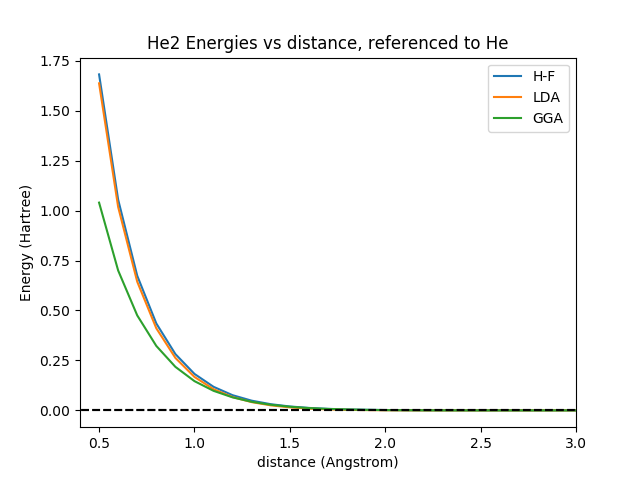
\includegraphics[width=.9\linewidth]{./Images/He2.png}
\end{center}

\subsection{Open-shell systems}
\label{sec:orga638905}
First, some jargon related to unpaired electrons:
\begin{center}
\begin{tabular}{rlrl}
\# unpaired electrons & \(S\) & \(2S+1\) & name\\
\hline
0 & 0 & 1 & singlet\\
1 & \(1/2\) & 2 & doublet\\
2 & 1 & 3 & triplet\\
3 & \(3/2\) & 4 & quartet\\
\end{tabular}
\end{center}

Model has to be generalized somewhat to deal with systems with unpaired electrons. One approach is to construct wavefunctions that are exactly spin-adapted (eigenfunctions of the \(\hat{S}\) operator). Possible in the Hartree-Fock world, but messy.  More common is to relax that constraint a bit, define different orbital wavefunctions for spin-up and spin-down electrons, called \emph{unrestricted} or \emph{spin-polarized} (opposite of \emph{non-spin-polarized}!).  Means that electron density has different spin-up and spin-down parts.

\begin{center}
\includegraphics[width=0.9\textwidth]{./Images/Polarization.png}
\end{center}

Controlled in \texttt{GAMESS} using the \texttt{\$CONTRL} group:
\begin{verbatim}
 $CONTRL SCFTYP = RHF   non-spin-polarized, default
         SCFTYP = UHF   spin-polarized
         MULT   = 1 (default), 2,...  spin multiplicity = 1 + number of unpaired electrons
         ICHARG = 0 (default), 1,...  net charge
 $END
\end{verbatim}

\subsection{Gaussian basis sets}
\label{sec:org30af5f9}
Gaussian functions (\(e^{-\zeta|\mathbf{r}|^2}\)) are the most popular choice for atom-centered basis sets.  They do not efficiently represent molecular wavefunctions, but one- and two-electron integrals in  WFT  can be solved analytically over Gaussians.

Other choices, like Slater functions (\(e^{-\zeta|\mathbf{r}|}\)) are possible but require numerical quadrature.

Gaussian basis sets have to be created for any given atom and must be used consistently within a set of calculations.

\begin{itemize}
\item \uline{Primitive} is a single Gaussian function, possibly multipled by a polynomial to look like
\emph{s}, \emph{p}, \ldots.  Defined by an exponent \(\zeta\) that determines how extensive (small \(\zeta\)) or compact
the function is.
\item \uline{Contraction} is a pre-set linear combination of several primitive Gaussians.
\item \uline{Basis set} is a predefined set of exponents and contraction coefficients appropriate
for some specific atom.
\end{itemize}

\subsubsection{Gaussian basis set nomenclature}
\label{sec:org6beafcf}
\begin{itemize}
\item \uline{Minimal basis} contains one contracted function for every atomic orbital. STO-3G is the
poster child.
\item \uline{Double zeta} contains two contracted functions for every atomic orbital
\item \uline{Split valence} is more common, single zeta in core, double zete in valence, typical of Pople basis sets, eg ``6-31G''
\item \uline{Triple-split valence} would be ``6-311G''
\item \uline{Spherical} vs \uline{Cartesian} determines whether a \emph{d} function have 6 or 5 parts (the sixth of which is an \emph{s}).
\item \uline{Polarization functions} are functions of one angular momentum greater than the highest angular momentum occupied states, eg \(p\) function for H, or \(d\) function for C. Important to capture the polarization of charge when atoms make molecules.  Arcane nomenclature, eg 6-31G(d,p) or 6-31G**.
\item \uline{Diffuse functions} are small exponent functions to describe anions or loosely bound electrons. Again argane nomenclature, eg 6-31+G(d,p). Yech.
\item \uline{Correlation consistent} and \uline{atomic natural orbital} are series of basis sets that are constructured to be efficient and to improve systematically.
\item \uline{Complete basis set} (CBS) limit is notion of extrapolating energies from a series of systematically improving basis sets.  Very common in high accuracy calculations.
\end{itemize}

\subsubsection{Standard basis sets in \texttt{GAMESS}}
\label{sec:org7d7094d}
Specified in \$BASIS group.  Some common choices, in increasing level of sophistication:

\begin{center}
\begin{tabular}{lll}
\hline
Name & Type & Flags\\
\hline
 & \textbf{Pople type} & \textbf{The most venerable and widely used}\\
STO-3G & Minimal & GBASIS=STO  NGAUSS = 3\\
3-21G & Split valence & GBASIS=N21  NGAUSS=3\\
6-31G(d) & Split valence polarized & GBASIS=N31 NGAUSS =6 NDFUNC=1\\
6-311+G(d,p) & Triple-split valence & GBASIS=N311 NGAUSS=6 NDFUNC=1 NPFUNC=1\\
 & polarized and augmented & DIFFSP=1\\
 &  & \\
 & \textbf{Polarization-consistent} & \textbf{Good for DFT}\\
PC0 & Split valence & GBASIS=PCseg-0      ISPHER=1\\
PC1 & Split valence polarized & GBASIS=PCseg-1      ISPHER=1\\
PC2 & Triple split double polarized & GBASIS=PCseg-22     ISPHER=1\\
 &  & \\
 & \textbf{Correlation-consistent} & \textbf{Good for MP2 and beyond}\\
cc-pVDZ & Split valence polarized & GBASIS=CC2\\
cc-pVTZ & Triple split double polarized & GBASIS=CC3\\
aug-cc-pvDZ & augmented with diffuse functions & GBASIS=ACC2\\
 &  & \\
 & \textbf{Effective core potentials} & \textbf{Good for treating heavy atoms}\\
SBKJC & Split valence + core potential & GBASIS=SBKJC\\
Hay-Wadt & Split valence + core potential & GBASIS=HW\\
\hline
\end{tabular}
\end{center}

Complicated field, which is why the old standards live on in routine calculations.  Optimal approach is to employ a \uline{composite model}, calibrated by someone else, with well defined set of basis functions and treatments of exchance and correlation.  A composite model pieces together results from a number of different calculations to estimate a higher accuracy model.

\subsection{Electron cores}
\label{sec:org336ce81}
Low energy ``core'' electrons typically don't participate in chemical bonding but can add substantially  to computational cost.  Generally seek approximations, especially  for heavy elements/metals.

Heart of approach is to partition an atom into core and valence parts.  Seek ways to
express the influence of the core on the valence without actually having to compute the
core. Essentially seek to write 
\[ \hat{v}^\text{ee} \approx \hat{v}^\text{ee,core} +
\hat{v}^\text{ee,val} \] 
where the core potential is some simpler, composite expression of
the influence of the core on the valence.  Typically take the electron cores as ``frozen''
in the pure atomic states, and express influence on valence through
 angular-momentum-dependent operators parameterized against accurate atomic calculations.  Goal is to recover valence wavefunctions with less effort.

\subsubsection{Relativistic effects}
\label{sec:org675f26d}
Relativistic kinetic energy is relativistic total energy minus the rest energy:
 \[T = \sqrt{p^2c^2 + m_0^2c^4} - m_0c^2\]
Taylor expanding about \(p^2 = 0\) gives the \uline{first-order mass-velocity correction}:
\[ T \approx \frac{p^2}{2m_0} - \frac{p^4}{8 m_0^3 c^2}\]
Reduces to non-relativistic result when \(c\rightarrow\infty\).  Electrons near core move at speeds close to \(c\), second term becomes non-negligible and diminishes their energy.  Most important for \(s\) states that penetrate closest to nucleus; they shield nucleus better and other valence states rise up in energy.

Electron spin and orbital magnetic moments also couple when \(l>0\), leads to \uline{spin-orbit coupling} that splits \(p\), \(d\), \ldots states into \(j = l \pm s\) states. 

\begin{figure}[htbp]
\centering
\includegraphics[width=.5\textwidth]{./Images/Relativity.png}
\caption{Comparison of Non-Relativistic and Relativistic Atomic States.}
\end{figure}

\uline{Darwin correction} corrects s orbitals for electron and nucleus being at the same point; comes from solution of full Dirac relativistic equation for the atom.

Relativistic effects typically incorporated implicitly, by including in model for core electrons and thus capturing their effect on the valence.  Spin-orbit, if necessary, added after the fact.
\subsubsection{Implementations}
\label{sec:org6be9e3f}
Non-relativistic and relativistic effective core potentials (ECPs) available for many elements.  These specify the potential felt by the valence electrons due to the core in terms of radial potential functions and angular projection operators.  Typically these have to be combined with basis functions designed to work with them.

Most common are Hay-Wadt (LANL) and Stevens-Basch-Krause (SBK).  Other more modern ones also available, like Stuttgart.

Essential to all plane-wave codes, like \texttt{Vasp}, but implemented differently.  Will touch on later in class.
\subsection{Population analysis}
\label{sec:org443e795}
The molecular orbitals contain information that can be helpful in understanding structure and bonding:  

\begin{itemize}
\item \uline{Charge density} most direct representation of electron distribution
\end{itemize}
\[ \rho(\bm{r}) = \sum_\text{occupied} |\psi_i(\bm{r})|^2 = \sum_{\mu,\nu}P_{\mu,\nu}\phi_\mu(\bm{r})\phi_\nu(\bm{r}) \]

\begin{itemize}
\item \uline{Moments} of charge density (dipole, quadrupole), useful for thinking about molecule-molecule interactions.  (Only exactly defined for neutrals!)

\item \uline{Electrostatic potential}, or Coulomb potential created by electrons and nuclei.  More refined way of thinking about ``how spots'' on a molecule. Commonly used to parameterize classical forcefields, by seeking set of atom-centered charges that reproduce calculated electrostatic potential, as is done with \texttt{CHELPG}.  Not uniquely defined.

\item \uline{Population analyses}, which attempt to distribute electrons to individual atoms and possibly bonds based on decomposition of molecular orbitals.  Chemically it is intuitively nice to assign charge to individual atoms.  There is no single ``right'' way to do this\ldots the ``charge'' on an atom in a molecule in not uniquely defined!  Consider an occupied molecular orbital \(\psi\) made up of two basis functions on two different atoms, \(\alpha\) and \(\beta\):
\end{itemize}
\begin{eqnarray}
\psi &=& c_\alpha \phi_\alpha + c_\beta \phi_\beta \\
\langle \psi | \psi \rangle &=& c_\alpha^2 + c_\beta^2 + 2 c_\alpha c_\beta \langle\phi_\alpha | \phi_\beta\rangle
\end{eqnarray}
In \emph{Mulliken} analysis, \(c_\alpha^2\) is fraction of \(\psi\) assignable to the atom of \(\alpha\), \(c_\beta^2\) fraction assigned to atom of \(\beta\).  Remainder is the ``overlap'' population, which is split evenly between the two.  Summing over all occupied orbitals and subtracting nuclear charges gives \emph{gross atomic charges}.

In \emph{L\"{o}wdin} analysis, basis functions are pre-orthogonalized, so last term vanishes.

Both approaches very sensitive to choice of basis set. Only sensible to compare within a common model type across molecules.

\begin{itemize}
\item \uline{Localized orbitals} is notion of creating linear combinations of \(\psi\) that satisfy some constraint for being compact. Leads to orbitals that are more naturally ``bonding.''

\item \uline{Natural orbitals} a rigorous scheme for orthogonalizing and assigning charge.  Based on recognition that there is a set of orthogonal orbitals that optimally describe the density.  Localizing these give \emph{natural bonding orbitals}.  See \href{./Resources/06Weinhold.pdf}{06Weinhold.pdf}.

\item \uline{Bader analysis} another method, based on a geometric analysis of the total charge density.  Define See Bader, R. F. W. Atoms in Molecules: A Quantum Theory; Oxford University Press: Oxford, 1990.
\end{itemize}
\subsection{Molecular orbital (MO) diagrams}
\label{sec:orgddf3604}
Correlate molecular orbitals with their parent fragments.  Use to be the thing.  Seldom now
\subsection{Implementation details of SCF methods}
\label{sec:org35584ae}
Basis is often \emph{orthonormalized} to eliminate overlap from H-F-R equation; allows equations to be solved by matrix diagonalization.

Initial density matrix \(\mathbf{P}\) are obtained by solving an approximate Hamiltonian (like extended H\"{u}ckel). Always beware! Initial guess can influence final converged state.

Because the number of 2-electron integrals grows as \(N^4\), they are sometimes calculated as needed ``on-the-fly'', so-called direct SCF.

Hartree-Fock integrals can be computed analytically in a Gaussian basis.  Any other choice of basis, or any DFT functional, requires integrals to be computed by quadrature. Used to be a real hang-up.  Today, algorithms are very robust to establish grids and do quadrature.
\subsection{SCF updating}
\label{sec:org5243f67}
The SCF procedure is an optimization problem: find set of coefficients that minimizes the total energy. As discussed above, success depends on a reasonable initial guess for density matrix and judicious updating. Various strategies can be used to speed and stabilize convergence, like damped mixing of previous cycles.

Second-order SCF is a convergence acceleration method that requires calculation or estimation of the first- and second-derivatives of the energy with respect to the orbital coefficients. See e.g. Chaban et al., \emph{Theor. Chem. Accts.} \textbf{1997}, \emph{97}, 88-95.

Pulay's ``direct inversion in the iterative subspace,'' or ``DIIS,'' is a popular and powerful acceleration procedure that extrapolates from several previous Fock matrices to predict optimal next Fock to diagonalize. \textbf{An opportunity for machine learning?} 

Controlled in GAMESS using the \texttt{\$SCF} group.

\begin{verbatim}
 $SCF DIRSCF=   .T./.F. controls direct scf
      SOSCF=    .T./.F. second-order scf
      DIIS=     .F./.T. direct inversion in the iterative subspace
      DAMP=     .T./.F. damping, on for initial iterations
 $END
\end{verbatim}

Can also control initial guess orbitals. Particularly powerful feature is to restart from converged orbitals from a previous calculations (.dat file), controlled with \texttt{\$GUESS} group.

\begin{verbatim}
 $GUESS GUESS = HUCKEL   construct intial guess from a simple Hamiltonian
              = MOREAD   read in orbitals from $VEC group.
\end{verbatim}


\newpage
\section{Potential energy surfaces}
\label{sec:org9ca9606}
The potential energy surface (``PES'') is the sum of the repulsive energy of the nuclei and the kinetic and potential energies of all the electrons:
\begin{center}
\begin{equation}
E_\text{PES}(\mathbf{R_\alpha},\mathbf{R_\beta},\ldots) =E_\text{elec} +\sum_{\alpha=1}^N \sum_{\beta =\alpha +1}^N \frac{Z_\alpha Z_\beta e^2}{R_{\alpha \beta}}
\end{equation}
\end{center}
\subsection{Specifying atomic positions}
\label{sec:orged99d2e}

\begin{center}
\begin{center}
\includegraphics[width=0.75\textwidth]{./Images/Internals.pdf}
\end{center}
\end{center}

\subsubsection{Cartesian}
\label{sec:orga60e60c}
Computationally straightforward but don't correspond with our physical notion of bonds,
bends, etc.  Easiest to get out of a piece of software.  A molecule has \(3 N-6\) internal degrees of freedom (\(3N-5\) if linear), but Cartesians specify \(3N\).  The extra values correspond to the location of the center of mass and molecular oriendation.  Codes will typically center and reorient the Cartesians.

In \texttt{GAMESS}, would specify Cartesian coordinates for \ce{FCH2CH2F} like this:
\begin{verbatim}
 $CONTRL COORD=CART $END
 $DATA
FCH2CH2F drag calculation
C1
C     6.0    -3.76764     0.33879     0.03727
C     6.0    -2.35246     0.34495     0.03689
F     9.0    -4.72277     0.58147    -1.18012
F     9.0    -1.59909    -0.68487    -0.83662
H     1.0    -4.04387     1.08375     0.75395
H     1.0    -3.92958    -0.71060     0.16941
H     1.0    -2.03786     0.18875     1.04760
H     1.0    -2.09983     1.28759    -0.40187
 $END
\end{verbatim}
\subsubsection{Internal coordinates}
\label{sec:org401e964}
These provide a more intuitive representation and can be convenient when building molecules by hand.  In codes like \texttt{GAMESS}, most commonly defined using ``z-matrix'' notation. Specify  each atom in terms of its distance, angle, and dihedral angle with three previous atoms.

In Gamess, would specify z-matrix for \ce{FCH2CH2F} like this:
\begin{verbatim}
$CONTRL SCFTYP=RHF RUNTYP=ENERGY COORD=ZMT $END
$DATA
FCH2CH2F drag calculation
C1
C
C   1   r1
F   2   r2   1   A1
H   2   r3   1   A2   3   D1
H   2   r4   1   A3   3   D2
F   1   r2   2   A1   3   D3
H   1   r3   2   A2   6   D1
H   1   r4   2   A3   6   D2

r1=1.5386
r2=1.39462
r3=1.11456
r4=1.12
A1=109.54214
A2=111.
A3=110.
D1=120.
D2=-120.5
D3=50.
$END
\end{verbatim}
Particularly convenient when you'd like to ``scan'' over the value of some coordinate.  Variable can be applied to more than one independent coordinate, if the molecule has symmetry.

\subsection{Features of potential energy surfaces}
\label{sec:orga2da390}
\subsubsection{One-dimensional example}
\label{sec:org482f0b0}
\begin{center}
\begin{center}
\includegraphics[width=0.75\textwidth]{./Images/PES.pdf}
\end{center}
\end{center}
Note 3-fold periodicity as expected for rotation about a \ce{C−C} single bond.  Note too there are some special points:

\begin{itemize}
\item \uline{Minima} are places where energy bottoms out.  More formally, first derivative of energy, or slope, or ``gradient'' \(g = 0\), and second derivative, or curvature, or ``Hessian'' \(H > 0\).  These are the \textbf{locally} stable conformations of the molecule.  Note that lowest energy in this case is not trans, but rather gauche conformations.  Are you surprised?

\item \uline{Saddle points} are places where energy is maximized.  Physicially, corresponds to ``transition states'' connecting low-energy conformations.  Gradient \(g = 0\), but curvature \(H < 0\).
\end{itemize}

\subsubsection{Many-dimensional PES features}
\label{sec:org156dde1}
Gradient becomes vector and Hessian a matrix

\[ \bm{g} = \left ( \begin{array}{c} \frac{\partial E}{\partial q_1} \\ \vdots \\ \frac{\partial E}{\partial q_{3N}} \end{array} \right )\qquad \bm{H} = \left (\begin{array}{ccc} \frac{\partial^2 E}{\partial q_1^2} & \cdots & \frac{\partial^2 E}{\partial q_1\partial q_{3N}} \\ \vdots & \ddots & \vdots \\ \frac{\partial^2 E}{\partial q_1\partial q_{3N}} & \cdots & \frac{\partial^2 E}{\partial q_{3N}^2}  \end{array} \right ) \]

\begin{figure}[htbp]
\centering
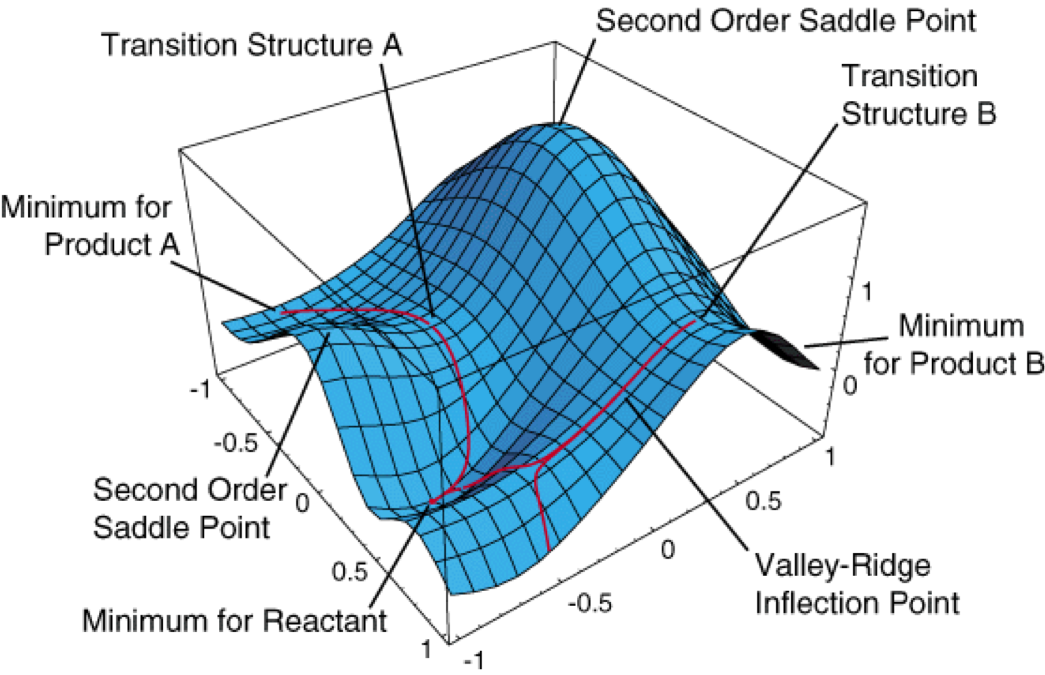
\includegraphics[width=0.75\textwidth]{./Images/Schlegel-PES.png}
\caption{From Schlegel, \emph{J. Comp. Chem.} \textbf{2003}, \emph{24}, 1514-1527.}
\end{figure}

\begin{itemize}
\item \uline{gradient} is vector tangent to PES.  The force on an object is \(\bm{F} = - \bm{g}\), so the gradients are often called the forces.  Where gradient (slope) is negative, force is positive, and vice versa.  Force always pushes system toward nearest minimum. If the potential is harmonic, then the force constant \(k = H\), so the Hessian is also called the ``force constant.''

\item \uline{Hessian matrix} is real and symmetric. Diagonalization gives eignevalues and eigenvectors.  Eigenvectors give ``natural'' directions along PES (physically, the harmonic vibrational modes), and eigenvalues indicate curvature in that direction.

\item \uline{Minimum} on multidimensional PES has gradient vector \(\bm{g} = 0\) and all positive Hessian eigenvalues.

\item \uline{First-order saddle point}, or \uline{transition state}, has \(\bm{g} = 0\) and one and only one negative Hessian eigenvalues.  (Physically, one unique direction that leads downhill in energy.)  Must correspond to lowest-energy point connecting two minima.

\item \uline{Minimum energy pathway} (MEP) or \uline{intrinsic reaction coordinate} (IRC) is steepest descent pathway (in mass-weighted coordinates) from saddle point to nearby minima.  Path a marble with infinite inertia would follow.

\item \uline{Higher order saddle points} have \(\bm{g} = 0\) and more than one negative Hessian eigenvalue.  Can always lead to lower energy first order saddle point.  These generally do not have chemical significance.
\end{itemize}

In computational chemistry/materials science, it is frequently  our job to identify the critical points (minima and transition states on a PES).  In liquids, PES much more flat and lightly corrugated.  Statistical mechanics becomes mores important.

Each distinct electronic state defines its own PES. Remember that there are multiple PES’s for any atom configuration, corresponding to different electronic states.  Sometimes these states can interact, intersect, giving avoided crossings, conical intersections.  Lead to more complicated dynamical behavior.

\subsection{Energy gradients and second derivatives}
\label{sec:orgb460b1a}
\subsubsection{Gradients}
\label{sec:orge58d9e8}
\[ \frac{\partial E_\text{elec}}{\partial q_i} = \frac{\partial}{\partial q_i} \langle \Psi | \hat{H} | \Psi \rangle = \langle \frac{\partial \Psi}{\partial q_i} | \hat{H} | \Psi \rangle + \langle \Psi |\frac{\partial \hat{H}}{\partial q_i} | \Psi \rangle + \langle  \Psi | \hat{H} | \frac{\partial \Psi}{\partial q_i} \Psi \rangle  \]
\begin{itemize}
\item \uline{Hellman-Feynmann theorem} says that sum of first and last terms vanish, so in principle only need to compute middle, which involves derivative of Coulomb potential and can be evaluated.
\item \uline{Pulay forces} are forces from first and last terms that appear when basis functions are centered on atoms.  An advantage of plane-wave basis sets, for which these terms vanish.
\end{itemize}
\subsubsection{Hessian}
\label{sec:org3563ba7}
In some electronic structure models can be computed analytically.  More commonly, determined from numerical differentiation of gradients.  Implementations typically assume that system is at minimum.

\begin{center}
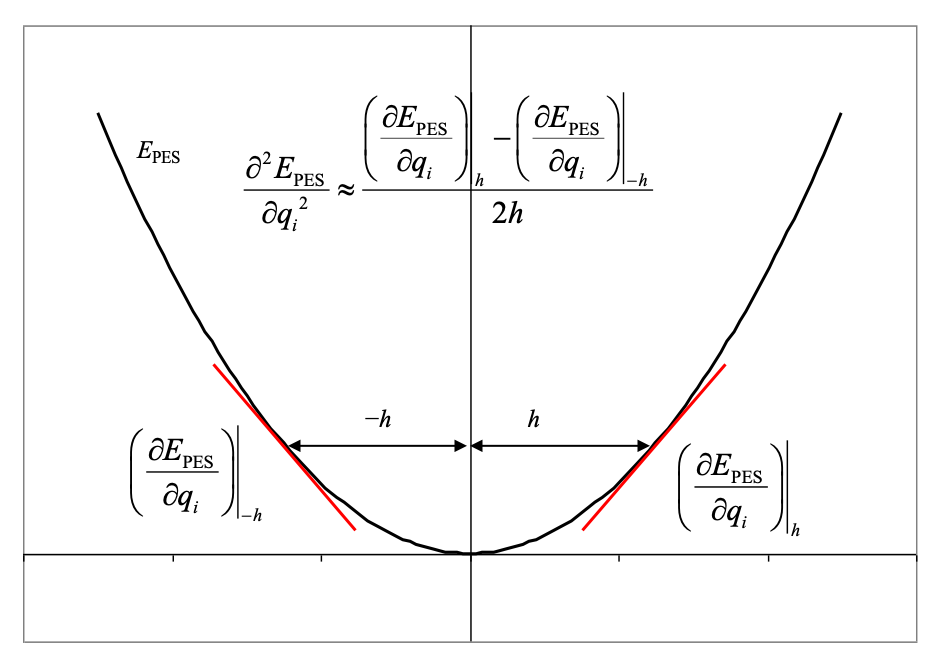
\includegraphics[width=0.5\textwidth]{./Images/Harmonic.png}
\end{center}

\emph{h} must be small enough to stay in the harmonic region, but big enough to avoid numerical noise swamping the gradients.  

For a molecule with \emph{N} atoms, to construct complete  \(3N\times  3N\) Hessian, have to evaluate gradients \(6N\) times for two-sided differencing.  Each pair of displacements completes one row of Hessian.  Obviously tends to be quite expensive.

To get better precision and accuracy, could calculate more than two displacements, and could fit to a more complicated function than a harmonic potential.

\subsection{Geometry optimization algorithms}
\label{sec:org9132528}
\subsubsection{Energy-only}
\label{sec:org78d7629}
\begin{itemize}
\item \uline{Trudge} infers gradient and locates minimum by wandering around
\end{itemize}
\subsubsection{Energy + gradient}
\label{sec:orgca247f9}
\begin{itemize}
\item \uline{Steepest descent}, just march down hill.  \(\bm{R}^\prime = \bm{R} - \lambda \bm{g}\). Safe, very inefficient near minimum. May do line search to adapt \(\lambda\).
\item \uline{Conjugate gradient} is steepest descent plus orthogonalization to previous step.  Safe, less very inefficient, common choice when far from minima.
\end{itemize}
\subsubsection{Energy + gradient + higher order}
\label{sec:orgc5ed909}
\begin{itemize}
\item \uline{Quasi-Newton Raphson} takes advantages of both first and second derivative information:
\[ \bm{R}^\prime = \bm{R} - \bm{H}^{-1}(\bm{R})\bm{g}(\bm{R}) \]
\end{itemize}
Typically do not know Hessian and it is expensive to calculate.  Make an initial guess, then update Hessian with gradient information from each geometry step. ``Learning'' PES as we go. Generally converges very rapidly near minima, where surface is not too anharmonic.
\begin{itemize}
\item \uline{Rational function optimization} is similar in spirit, also constructs Hessian, but uses more sophisticated (than quadratic) guess form of PES to update positions.
\item \uline{Direct inversion in the iterative subspace} (DIIS) uses sizes of QNR steps as estimates of error and constructs new step from linear combination of previous that minimizes error inferred from previous steps:
\[ \bm{err}(\bm{R}) = \sum_i c_i \bm{H}^{-1}_i \bm{g}_i \]
\end{itemize}
Generally very efficient in region of minimum. Algorithm can misbehave away from minima, possibly even converging to nearby saddle points, so often started with conjugate gradient steps. 
\subsubsection{Machine learning}
\label{sec:org9a27eab}
All of these based on some form of assumed model of underlying PES (Taylor expand to second order around minimum).  Emerging are methods that ``fingerprint'' structure and construct and improve energy model with each step. Remains to be seen if a new ``standard'' emerges. 
\subsubsection{Global optimizations}
\label{sec:orgb437b0c}
Simulated annealling, genetic algorithms, \ldots, more on the exotic side.
\subsubsection{Convergence criteria}
\label{sec:org910caf0}
Typically determine convergence by enforcing maximum on each individual force component 

\texttt{GAMESS} offers a limited set of algorithms.
\begin{verbatim}
 $STATPT METHOD = NR     ! Quasi-Newton Raphson
                = RFO    ! rational function optimization
         OPTTOL = 0.0001 ! convergence criterion in au/bohr.
         HESS = GUESS    ! guess an initial Hessian
              = READ     ! read from $VIB group
 $END
\end{verbatim}

\subsection{Specify \texttt{GAMESS} calculation type}
\label{sec:orge1f3f59}
Specified in \$CONTRL group by RUNTYP flag:

\begin{center}
\begin{tabular}{ll}
Calculation & RUNTYP=\\
\hline
Single-point energy & Energy\\
Single-point energy + force & Gradient\\
Geometry optimization & Optimize\\
Linear scan over PES & Scan\\
Energy + second derivative & Hessian\\
Transition state search & Sadpoint\\
Intrinisc reaction coordinate & IRC\\
\end{tabular}
\end{center}

Note too that specifying EXETYP=CHECK will check your input without actually running the job.

Hessian (force) calculation can be done analytically or by numerical differentiation of forces, depending on electronic structure method:
\begin{verbatim}
 $FORCE METHOD = ANALYTICAL
               = SEMINUM
        VIBSIZ = 0.01    ! step size (bohr)
 $END
\end{verbatim}

\subsection{Efficient coordinate systems}
\label{sec:orgcb02e5d}
Optimizations are most efficient in coordinate system that diagonalizes Hessian, so that optimizations along each direction are (nearly) independent.  Large off-diagonal Hessian terms imply strong coupling.  Cartesian coordinates do not reflect physical forces in system and are generally poor choice/slow convergence for optimizations. Can choose other coordinate systems. Forces/Hessian always computed in cartesians, so any other coordinate system requires transformations back and forth.

\begin{itemize}
\item \uline{Cartesians} simplest to implement, consistent performance.  Typically only choice in supercell calculations.

\item \uline{Z-matrix} are easy to define and use for organic molecules with no rings.  For \(3N-6\) degrees of freedom, must specify \(N-1\) distances, \(N-2\) angles, and \(N-3\) dihedrals.  Typically will converge much faster than Cartesians for small molecules.  Implemented in most molecular codes, including \texttt{GAMESS}.
\end{itemize}

\begin{verbatim}
 $CONTRL COORD=ZMAT NZVAR = 3N-6 $END
\end{verbatim}

\begin{itemize}
\item \uline{Natural internals} are generalizations of z-matrix that are coordinates that approximately diagonalize Hessian. Hard to generate \emph{a priori} or automatically. Specification in \texttt{GAMESS} is arcane, done in \texttt{\$ZMAT}.

\item \uline{Redundant internals} are an over-determined set of internal coordinates, like all bond distance, all angles between bonded atoms, all dihedrals.  Easily constructed automatically. Mapping between Cartesians and redundant internals becomes more complicated; transform from redundant to Cartesians is overdetermined and has to be solved iteratively.  Works very efficiently for molecules though. Implemented (in spirit) in \texttt{GAMESS}.
\end{itemize}
\begin{verbatim}
 $CONTRL NZVAR = 3N-6 $END
 $ZMAT DLC=.TRUE.  AUTO=.TRUE. $END
\end{verbatim}

\begin{center}
\begin{tabular}{lrl}
\hline
 & FCH2CH2F & C5H10\\
\hline
Cartesian & 13 & 30\\
Z-matrix & 11 & failed\\
Redundant/DLC & 16 & failed\\
\end{tabular}
\end{center}

\subsection{Performance of models for geometries}
\label{sec:orgf454f22}
Generally pretty good!  Gross geometries of molecules can be computed with good reliability using common approximations (H-F, LDA, GGA). Subtler things (does \ce{FCH2CH2F} really prefer \emph{trans} or \emph{gauche}?) can take more care in choice of electronic structure model. \url{https://cccbdb.nist.gov/} is a great place to look for benchmarks.

\subsection{Vibrational frequencies}
\label{sec:org3393a2b}
Suppose we are at a minimum on a PES.  Near that minimum, we can Taylor expand the PES and truncate at second order (``harmonic'', or quadratic, approximation).  The Schr\"{o}dinder equation describing the dynamical motion of the nuclei can be written in terms of displacements from the equilibrium position, \(q_i = x_i - x^\text{eq}_i\), \(i =1, \ldots, 3N\) and the Hessian \(H\):
\[\hat{H} = -\frac{\hbar^2}{2}\sum_i \frac{1}{m_i}\frac{\partial^2}{dq_i^2}+\frac{1}{2}\sum_{i,j} H_{ij} q_i q_j\]
or in mass-weighted coordinates, \(\xi_i=\sqrt{m_i}q_i\):
\[ \hat{H} = -\frac{\hbar^2}{2}\sum_i \frac{\partial^2}{d\xi_i^2}+\frac{1}{2}\sum_{i,j} \tilde{H}_{ij} \xi_i \xi_j,\qquad \tilde{H}_{ij}=\frac{1}{\sqrt{m_i m_j}}H_{ij} \]
From eigenvalues \(\kappa_i\) and eignevectors \(s_i\) (``normal modes'') of mass-weighted Hessian, can transform into \(3N\) one-dimensional problems:
\[\hat{H}_i=-\frac{\hbar^2}{2}\frac{d^2}{ds_i^2}+\kappa_is_i^2\]
This is one-dimensional harmonic oscillator Hamiltonian, solutions well known.
\begin{table}[]
   \begin{center}
   \caption{Harmonic oscillator model}
    \label{Harmonic-oscillator}
\begin{tabular}[h]{|c|}
\hline
 \\
$\displaystyle       V(x) = \frac{1}{2} \kappa x^2, -\infty < x < \infty $ \\
 \\
$\displaystyle     \psi_v(x) = N_v H_v(x/\alpha)e^{-x^2/2\alpha^2}, v = 0, 1, 2, \ldots $ \\
\\
$\displaystyle \alpha=(\hbar^2/\kappa)^{1/4}, N_v=(2^vv!\alpha\sqrt{\pi})^{-1/2} $ \\
 \\
\underline{Hermite polynomials} \\
$\displaystyle H_0(y) =1$\\
$\displaystyle H_1(y) = 2y$\\
$\displaystyle H_2(y) = 4y^2-2$\\
$\displaystyle H_{n+1}(y) = 2 y H_n(y) -2 n H_{n-1}(y)$\\
 \\
$\displaystyle     \nu =\frac{1}{2\pi}\sqrt{\kappa}$ \\
$\displaystyle     E_v=\left (v+\frac{1}{2}\right )h \nu, v=0, 1, 2, ...$ \\
% \\
%     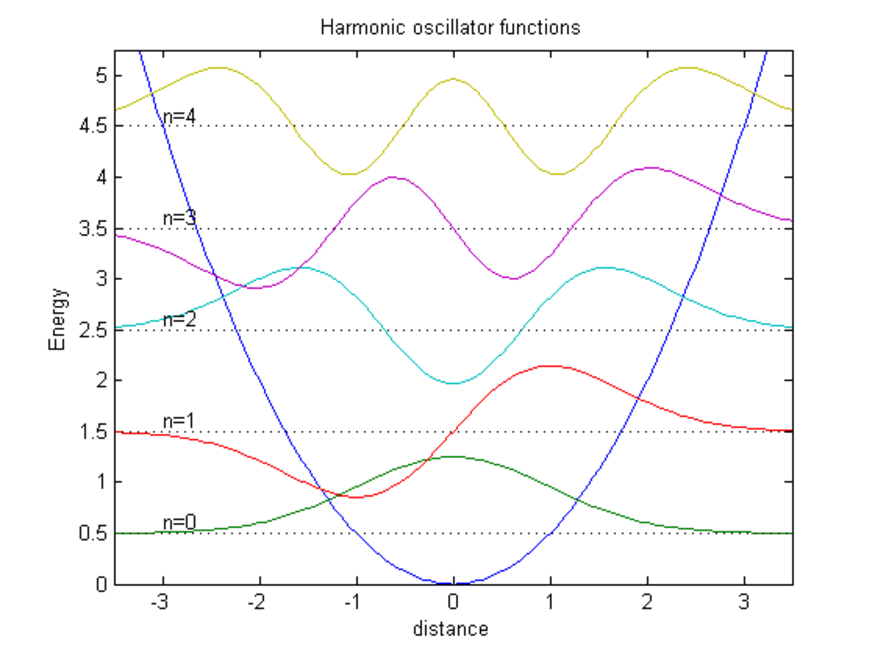
\includegraphics[scale=.6]{./Images/HO} \\       
\hline
\end{tabular}
 \end{center}
\end{table}

\begin{center}
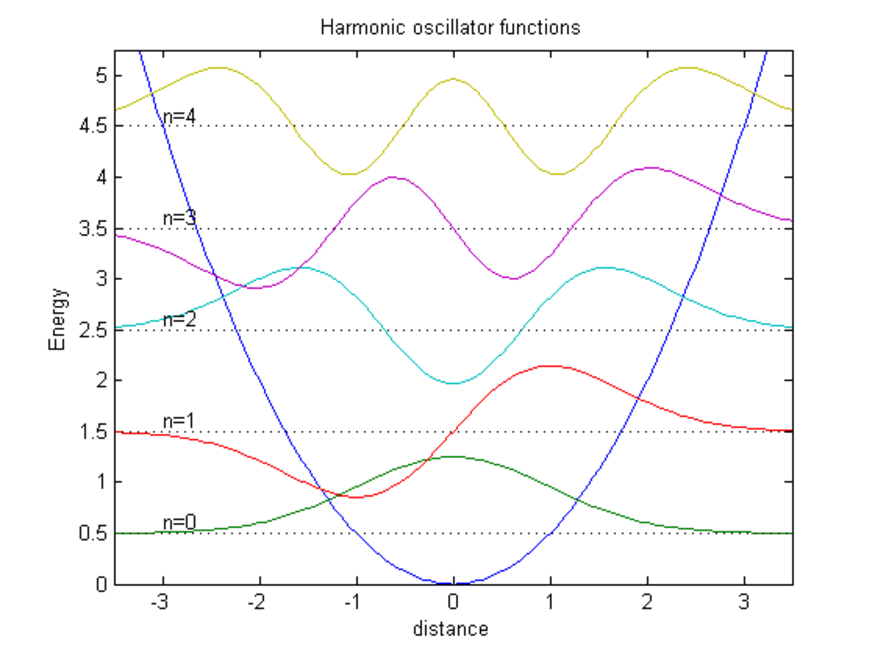
\includegraphics[width=0.5\textwidth]{./Images/HO.pdf}
\end{center}

Do this in \(3N\) Cartesian space, so 6 (or 5) of the normal modes correspond to translations and rotations of the molecule.  If calculation is exact, these will have \(\kappa_i = 0\).  Numerical errors may make them somewhat non-zero.  If necessary, these can be projected out by transforming Hessian to internal and back to Cartesian coordinates.

Note it is impossible for molecule to just sit at \(q = 0\).  Nuclei are \emph{always vibrating} about \(x^\text{eq}\). Gives zero point energy
\[ZPE = \frac{1}{2}\sum_i h\nu_i\]

For a chemical bond, \(\kappa\approx \SI{500}{N.m^{-1}}\), \(h\nu \approx \SI{0.8}{eV}\).

\subsubsection{Absorption intensities}
\label{sec:orgaaec210}
Vibrational modes can be probed/observed spectroscopically.  Intensity of stimulated absorption from vibrational state \emph{i} to \emph{f} given by Einstein coefficient of stimulated absorption:
\[B_{if}=\frac{|\mu_{if}|^2}{6\epsilon_0\hbar^2}\]
Arises from coupling of electric field of light with dipole of system.  Transition dipole moment, \(\mu_{if})\, given by:
\[\mu_{if} = \langle \psi_i|\hat\mu |\psi_f \rangle\]
where \(\hat\mu\) is dipole operator, 
\[\hat\mu = \sum q_i \bm{r}_i \]
where sum runs over all charged particles and \(q_i\) is each charge.  Dipole moment changes as molecule vibrates.  In direction \(\xi\), can write
\[\hat\mu(\xi(t)) = \mu(0) +\xi(t)\left( \frac{d\mu}{d\xi}\right )_{\xi=0} + \ldots\]
Use harmonic oscillator wavefunctions for \(\psi_i\) and \(\psi_f\):
\[\mu_{if} = \langle \psi_i|\hat\mu |\psi_f \rangle = \langle \psi_i|\mu(0) |\psi_f \rangle + \left( \frac{d\mu}{d\xi}\right )_{\xi=0} \langle \psi_i | \xi|\psi_f\rangle + \ldots\]
First integral vanishes for \(i\ne f\). Second integral provides \emph{gross selection rule} that intensity of transition proportional to the \emph{dynamic}  dipole moment along vibrational normal mode \(\xi\) and \emph{particular selection rule} that intensity of transition is zero unless \(f = i \pm 1\).  Latter comes from nature of Hermite polynomials.  At normal temperatures, \(i = 0\), and the only observable vibrational transitions are \(1\rightarrow 2\).

\subsubsection{Performance of harmonic approximation for vibrational spectrum}
\label{sec:org059fed8}
Harmonic vibrational frequency systematically overestimate experiment. Convolution of \emph{harmonic approximation} error: actual PES is not exactly harmonic, and errors intrinsic to electronic structure model.  Errors are typically systematic (see eg \url{https://doi.org/10.1021/jp960976r}).

\begin{center}
\begin{tabular}{lr}
 & scale factor\\
\hline
HF/3-21G & 0.9085\\
HF/6-31G(d) & 0.8929\\
MP2/6-31G(d) & 0.9434\\
B3LYP/6-31G(d) & 0.9613\\
\end{tabular}
\end{center}

Relative intensities are generally predicted with good reliability.  Model predicts absorption peaks to be delta functions.  Peaks always broadened due to a variety of fundamental and instrumental considerations.  Common in displaying spectra to arbitrarily broaden using a Lorentzian function.

\begin{figure}[htbp]
\centering
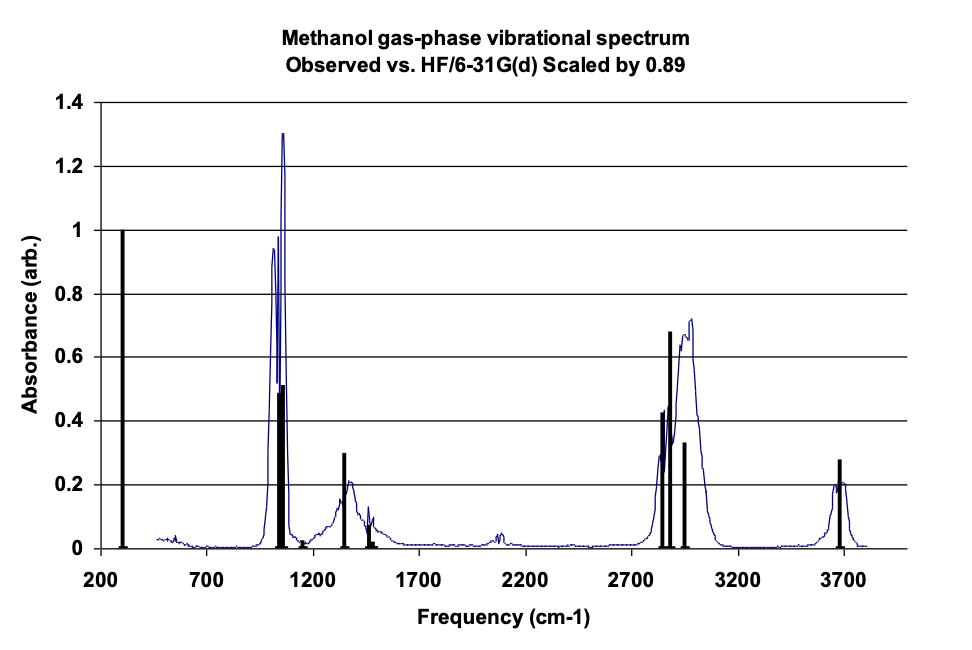
\includegraphics[width=0.75\textwidth]{./Images/Methanol.png}
\caption{Scaled HF/6-31G(d) vibrational spectrum vs experiment}
\end{figure}
\subsection{Transition states}
\label{sec:org3e68d3e}
\subsubsection{Symmetry}
\label{sec:org5f56ea9}
Can exploit symmetry to force calculation to converge to a transition state. Eclipsed form of \ce{FCH2-CH2F} has mirror symmetry (\(C_s\)), if initialized in that configuration, optimization must preserve symmetry.  

\begin{verbatim}
 $DATA
  FCH2CH2F eclipsed z-matrix (Cs, or mirror, symmetry)
CS

 C   
 C      1   1.5000000
 F      2   1.4000000  1   109.5421400
 H      2   1.1000000  1   109.5421400  3   120.0000000  0
 H      2   1.1000000  1   109.5421400  3  -120.0000000  0
 F      1   1.5000000  2   109.5421400  3     0.0000000  0
 H      1   1.1000000  2   109.5421400  6   120.0000000  0
 H      1   1.1000000  2   109.5421400  6  -120.0000000  0
 $END
\end{verbatim}

See results in \url{../Labs/Gamess/FCH2CH2F/SYMMETRY}.

\begin{center}
\begin{tabular}{ccc}
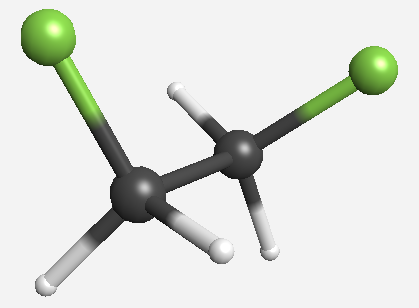
\includegraphics{./Images/FCH2CH2F-gauche.png}
 & \(\longrightarrow\) & 
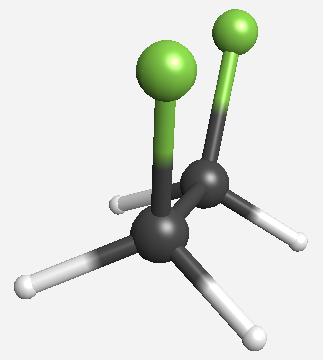
\includegraphics{./Images/FCH2CH2F-eclipsed.png} \\
\SI{-277.9377770749}{au} &  & \SI{-277.9253478441}{au} \\
  &  \(\Delta E =\) \SI{0.34}{eV} &  \\
\end{tabular}
\end{center}

\subsubsection{Coordinate drag}
\label{sec:org6e5d637}
If reaction state coordinate maps closely onto some internal coordinate, then can do a series of ``constrained'' optimizations, fixing the coordinate of interest to a series of values and relaxing all other coordinates.  Use \texttt{IFREEZ} within \texttt{GAMESS}.  For example, define \ce{FCH2CH2F} using z-matrix and freeze \ce{F-C-C-F} dihedral angle at a series of values.

\begin{verbatim}
 $CONTRL SCFTYP=RHF DFTTYP=PBE RUNTYP=OPTIMIZE COORD=ZMT NZVAR=18 ISPHER=1 $END
 $BASIS GBASIS=PCseg-1 $END
 $STATPT IFREEZ(1)=12 $END
 $DATA
FCH2CH2F eclipsed TS
C1
C
C   1   r1
F   2   r2   1   A1
H   2   r3   1   A2   3   D1
H   2   r4   1   A3   3   D2
F   1   r5   2   A4   3   D3
H   1   r6   2   A5   6   D4
H   1   r7   2   A6   6   D5

...
D4=120.
...
 $END
\end{verbatim}

See results in \href{../Labs/Gamess/FCH2CH2F/SCAN}{../Labs/Gamess/FCH2CH2F/SCAN}.

\begin{figure}[htbp]
\centering
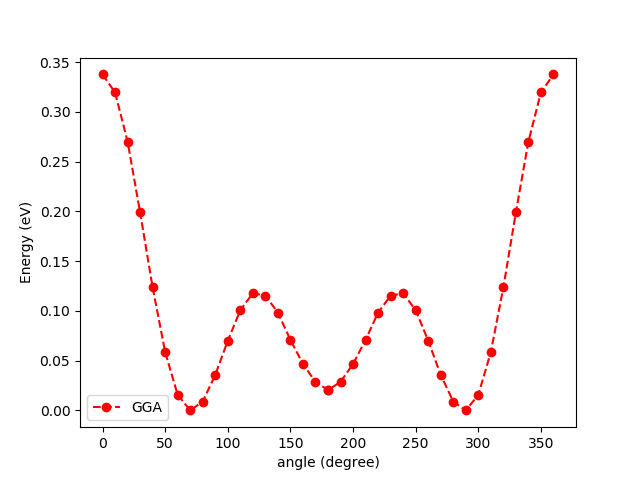
\includegraphics[width=0.75\textwidth]{./Images/FCH2CH2F-scan.png}
\caption{GGA/PCseg-1 rotational scan}
\end{figure}

A quasi-NR optimization started at one of the approximate TS's will usually converge to the exact TS.  
\begin{verbatim}
 $CONTRL SCFTYP=RHF DFTTYP=PBE RUNTYP=OPTIMIZE COORD=ZMT NZVAR=18 ISPHER=1 $END
 $STATPT METHOD=NR $END
 $BASIS GBASIS=PCseg-1 $END
 $DATA
FCH2CH2F zmatrix optimization near saddle point, no hessian
C1
 C   
 C      1   1.5256029
 F      2   1.4018052  1   110.3919125
 H      2   1.1066523  1   112.5759655  3   119.5903058  0
 H      2   1.1070172  1   108.5521191  3  -119.1579857  0
 F      1   1.4018888  2   110.3079213  3   120.0000000  0
 H      1   1.1065092  2   112.5372024  6   119.5247291  0
 H      1   1.1069911  2   108.5976341  6  -119.1645584  0
 $END
\end{verbatim}


See results in \href{../Labs/Gamess/FCH2CH2F/QNR-TS}{../Labs/Gamess/FCH2CH2F/QNR-TS}.  Always good practice to follow up with a frequency calculation to confirm.  

\begin{center}
\begin{tabular}{ccc}
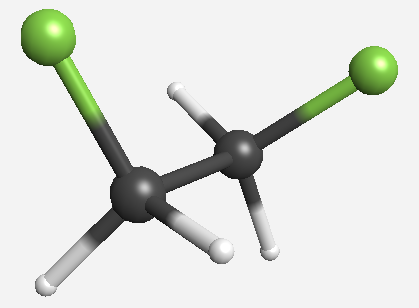
\includegraphics{./Images/FCH2CH2F-gauche.png}
 & \(\longrightarrow\) & 
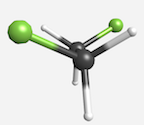
\includegraphics{./Images/FCH2CH2F-TS.png} \\
\SI{-277.9377770749}{au} &  & \SI{-277.9333073294}{au} \\
  &  \(\Delta E^\ddagger =\) \SI{0.12}{eV} &  \\
  &  \(\nu = 154i~\text{cm}^{-1}\) & \\
\end{tabular}
\end{center}

Coordinate dragging can fail when the reaction coordinate is non-linearly related to the multiple internal coordinates. Plus, it is relatively expensive, as it involves a lot of optimizations.
\subsubsection{1st order methods (NEB, \ldots{})}
\label{sec:org35152c3}
A scan is a first order method that freezes the gradient along a search direction.  A better algorithm would use the information along the search direction to find the TS and the entire MEP.  That's the spirit of a \emph{nudged elastic band} calculation, for instance. Also of newer methods to generate more sophisticated approximations.   Touch on that later\ldots{}.
\subsubsection{2nd order methods}
\label{sec:orgc1fb64f}
Hessian-based methods (like quasi-NR and DIIS) generally work more efficiently, assuming you can find a region reasonably close to the TS and can get a good guess of the Hessian with the appropriate (1!) number of negative eigenvalues.  These work like regular optimization methods, but search uphill along the negative eigenvector and downhill along the other directions.  The Hessian update scheme has to be appropriately modified to accommodate the negative eigenvalue.  The choice of coordinate system can become even more crucial.

Algorithm:
\begin{enumerate}
\item Identify and optimize structures of reactant and product states
\item Guess a structure for the TS, interpolated either mathematically or empirically between reactant and product
\item Compute initial TS Hessian (\texttt{RUNTYP = HESSIAN}).  Only needs to be approximately correct, so appropriate to use a less-expensive method.
\item Confirm Hessian has desired number of imaginary modes, or at least an imaginary mode that maps well onto desired reaction coordinate.
\item Do saddle-point search with guessed Hessian (\texttt{RUNTYP=SADPOINT}, \texttt{HESS=READ}).
\item Check result with final Hessian calculation
\end{enumerate}

\begin{verbatim}
 $CONTRL SCFTYP=RHF DFTTYP=PBE RUNTYP=SADPOINT COORD=CART ISPHER=1 $END
 $BASIS GBASIS=PCseg-1 $END
 $FORCE HESS=READ $END
 $DATA  
H2ON2                                                                           
C1       1
N           7.0      0.9405942384     -0.3241591975     -0.0156283505
N           7.0      0.0107640781      0.6540868381      0.0152029180
O           8.0     -0.9317086136     -0.2406652788     -0.0189127039
H           1.0     -0.2853795803     -0.9336844866      0.3015543918
H           1.0      1.8537652825      0.1690870887      0.0045149723
 $END      
 $HESS
ENERGY IS     -184.6737814637 E(NUC) IS       74.1740447013
 1  1 8.31017204E-01 1.46125961E-01 7.06555414E-04-1.42105871E-01 2.88851646E-02
 1  2-1.06097190E-03-3.64083936E-01 2.22079857E-02-2.60487424E-03-3.19838288E-02
.....
 $END
\end{verbatim}

See Results in \url{../Labs/Gamess/H2NNO-TS}.

\begin{center}
\begin{tabular}{ccccc}
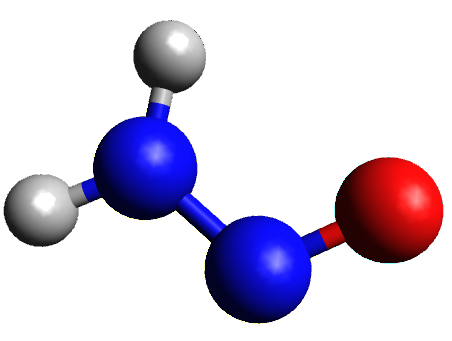
\includegraphics[width=0.22\textwidth]{./Images/H2NNO.png}
 & \(\longrightarrow\) & 
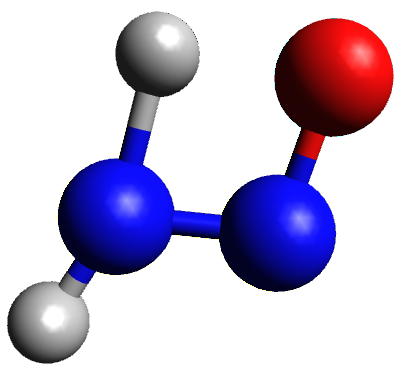
\includegraphics[width=0.22\textwidth]{./Images/H2NNO-TS.png} & \(\longrightarrow\) & 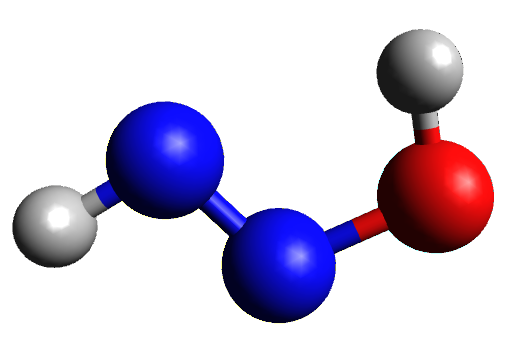
\includegraphics[width=0.22\textwidth]{./Images/HNNOH.png} \\
\SI{-185.6307937}{au} &  & \SI{-185.5854209}{au} & & \SI{-185.6254878}{au}\\
  &  \(\Delta E^\ddagger =\) & & \(\Delta E =\) \\
  &  \SI{1.23}{eV} & &  \SI{0.14}{eV} \\
\end{tabular}
\end{center}

\subsubsection{Well climbing}
\label{sec:org9befd86}
Algorithms exist that will climb out of basins and seek transition states\ldots{}.
\subsection{Intrinsic reaction coordinates}
\label{sec:org1876c4e}
In more complicated systems, it can often be difficult to know exactly what minima a particular transition state corresponds to. The intrinsic reaction coordinate (IRC) or minimum energy path (MEP) is steepestdescent path from TS towards both basins. Starts from TS, steps forward in direction given by gradient, using second order method. Have to use care in selecting algorithm and step sizes to stay on the path. Can be useful for locating variational transition state\ldots{}configuration where free energy (rather than energy) is maximized. 

\begin{verbatim}
 $CONTRL SCFTYP=RHF DFTTYP=PBE RUNTYP=IRC COORD=UNIQUE ISPHER=1 $END
 $BASIS GBASIS=PCseg-1 $END
 $IRC PACE=LINEAR STABLZ=.TRUE. NPOINT=10 SADDLE=.T. FORWRD=.T. $END
 $FORCE HESS=READ $END
 $DATA
H2ON2                                                                           
C1       1
 N           7.0   0.9233485039  -0.2399318160   0.0736256617
 N           7.0  -0.0272197420   0.6088503884  -0.0717581187
 O           8.0  -1.0933769256  -0.1081391759   0.0571959479
 H           1.0  -0.1059622027  -1.0519964547   0.2191639975
 H           1.0   1.8912457716   0.1158820221   0.0085037392
 $END      
 $HESS
ENERGY IS     -185.5854194050 E(NUC) IS       73.0033764178
 1  1 8.43287379E-01-4.86363743E-02 1.07610516E-04-3.07227749E-01 1.52208588E-01
.....
\end{verbatim}

\begin{center}
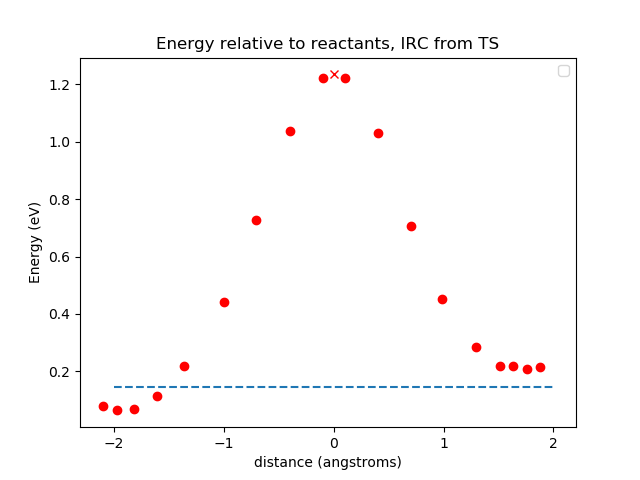
\includegraphics[width=.9\linewidth]{./Images/IRC.png}
\end{center}

\subsection{Molecular dynamics}
\label{sec:orgadf91e1}
Basic idea is to propogate atoms forward in time using some model to compute the forces on atoms and Newton's laws to describe kinetic energy of atoms.  May be done at constant energy (\emph{NVE}) or, by coupling kinetic energy to an appropriate reservoir, at constant temperature (\emph{NVT}).  Details beyond this course (perhaps beyond this instructor!).  Primary point for us is that cost of electronic structure calculations is great enough that typically some adjustments must be made to make force calculations cheap and fast enough to support number of evaluations necessary to do meaningful dynamics.
\subsubsection{Cheap parameters}
\label{sec:org85f3336}
Simplest trick is to back off on the precision and accuracy of calculations to reduce force evaluation cost.
\subsubsection{Car-Parrinello dynamics}
\label{sec:org8c56357}
Treat wavefunction itself as a dynamical variable and propogate forward in time along with the nuclei. Ideally parallels but does not exactly follow Born-Oppenheimer energy surface.  Huge advance when originally introduced, has fallen out of favor as more conventional B-O approaches compete more effectively.
\subsection{Biased sampling}
\label{sec:orga3d8462}
Ask Whitmer.  See \url{https://doi.org/10.1021/acs.jctc.8b00192}.
\newpage

\section{WFT Beyond Hartree-Fock}
\label{sec:orgc675e18}
DFT or WFT calculations of PES's are expensive.  Not uncommon to use an heirarcy of methods:
\begin{enumerate}
\item Characterize PES using some low-cost model (LDA)
\item Improve structures using some more reliable and expensive method
\item Improve final energies using some even more reliable and expensive method
\end{enumerate}

WFT has the advantage of offering a series of systematically improving models. Starts with Hartree-Fock ground-state wavefunction and build in ``many-body'' features/electron correlation by combining with ``excited'' Hartree-Fock wavefunctions:

\begin{center}
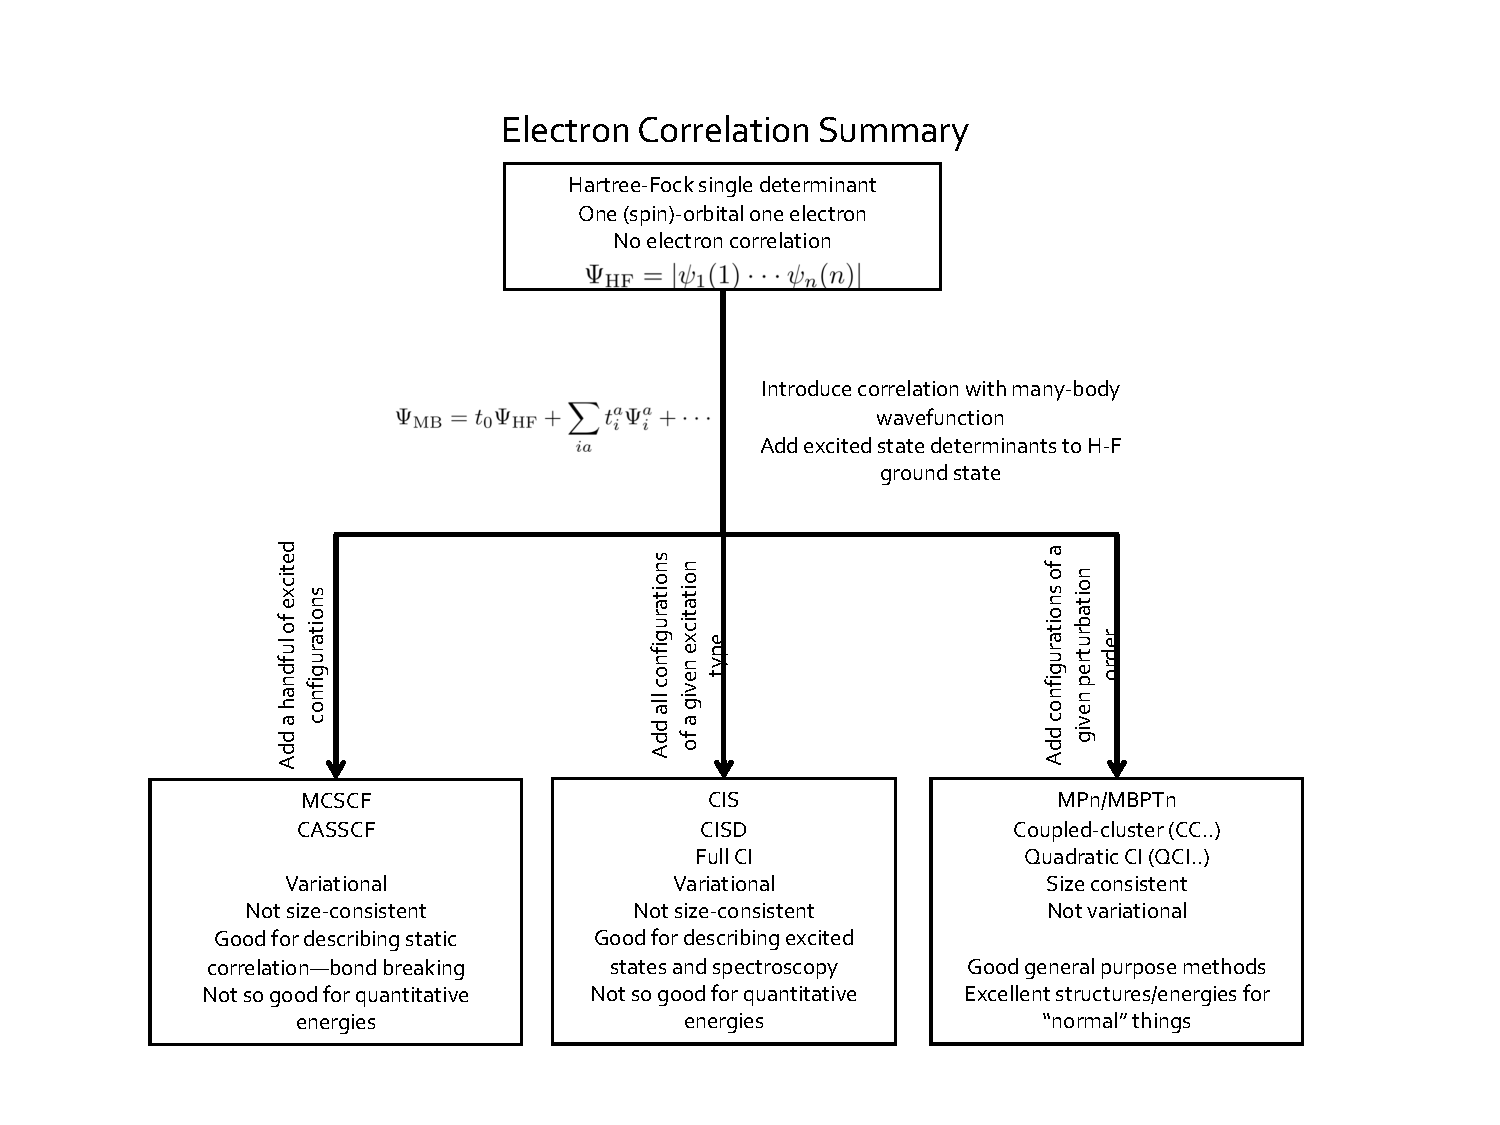
\includegraphics[width=1.0\textwidth]{./Images/correlation-summary.pdf}
\end{center}

\begin{itemize}
\item \uline{static correlation} are electron correlation effects that arise from the restrictive form of the H-F wavefunction
\item \uline{dynamic correlation} is like it sounds, the ``dance'' of all electrons about one another
\item \uline{configuration interaction} is a variational approach to adding in dynamical correlation by combining H-F determinants. Difficult to apply, rarely used any more.
\item \uline{size consistency} is the property that the energy model scales properly with the system size.  CI lacks this.
\item \uline{perturbation theory} (MPn) is non-variational, size-consistent, and user-friendly approach
\item \uline{coupled-cluster} (CCxxx) is a systematic, size-consistent approach to introducing H-F correlation.  Improvement on perturbation theory.
\item \uline{quadratic configuration interaction} (QCIxxx) is an approximate coupled cluster model.
\end{itemize}

Heirarcy of models:
\begin{center}
HF < MP2 \textasciitilde{} MP3 \textasciitilde{} CCD < CCSD < MP4 < CCSD(T) \textasciitilde{}
\end{center}
Reliability also tied to basis set completeness.

\begin{center}
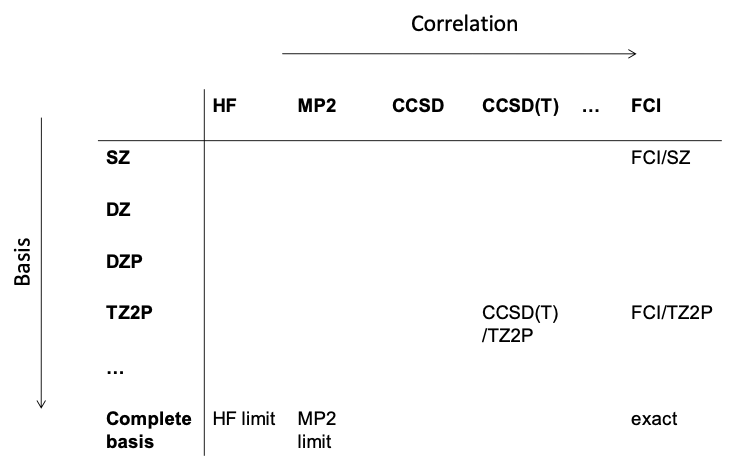
\includegraphics[width=.9\linewidth]{./Images/model-chem.png}
\end{center}

``Model chemistry'' some linear combination of these, often calibrated against experimental data. ``G2'' most venerable:

\begin{center}
\begin{tabular}{llrrr}
 & Hartree-Fock & MP2 & MP4 & QCISD(T)\\
\hline
6-31G(d) & ZPE & Structure &  & \\
6-311G(d) &  & 1 & 2 & 3\\
6-311+G(d,p) &  & 4 & 5 & \\
6-311G(2df,p) &  & 6 & 7 & \\
6-311+G(3df,p) &  & 8 &  & \\
\end{tabular}
\end{center}

\[ \text{QCISD(T)/6-311+G(3df,p)} \approx 2 + (3-2) + (5-2) + (7-2) + (8-1) - (4-1) - (6-1)\]
\[ \Delta E(\text{HLC}) = \SI{-2.50}{mHa} * (\text{# electron pairs}) - \SI{0.19}{mHa}* (\text{# unpaired electrons}) \]
\[ E(\text{G2}) = \text{QCISD(T)/6-311+G(3df,p)} + 0.8929 * \text{ZPE} + \Delta E(\text{HLC})\]

Quality assessed using, eg, mean absolute deviation from some reliable data set. Many elaborations on this same idea in the literature.

\newpage
\section{First-principles thermodynamics}
\label{sec:org30f7898}
\subsection{Connection Between QM and Thermodynamics}
\label{sec:orgd4a332d}
\subsubsection{Internal energy}
\label{sec:org775d9c6}
The \emph{internal electronic energy} of a single molecule from a WFT/DFT calculation is the energy
associated with taking infinitely separated constituent nuclei and electrons at
rest and forming a molecule:
\begin{equation}
2~\mathrm{H}^+ + 8~\mathrm{O}^{8+} + 10~\mathrm{e}^- \rightarrow
\mathrm{H_2O}\qquad E^\mathrm{elec}
\end{equation}
Calculate \(E^\mathrm{elec}\)  within the Born-Oppenheimer
approximation, so the nuclei are fixed in space
at the minimum energy configuration.  
\subsubsection{Zero-point vibrational energy}
\label{sec:orgc26b475}
\begin{equation}
  E^0=E^\mathrm{elec} + ZPVE
\end{equation}
ZPVE can be calculated reliably within the harmonic approximation, according to
\begin{equation}
  \mathrm{ZPVE}=\frac{1}{2}h\sum_{i=1}^{3n-6}\nu_i
\end{equation}
where \(\nu_i\) are the harmonic vibrational frequencies, obtained from a
vibrational frequency analysis.  \(E^0\) is the minimum physically meaninfful
energy of the molecule.
\subsubsection{Finite \emph{T} energy}
\label{sec:orgb0c49b2}
Energy can be deposited in a syste  as
translational and rotational kinetic energy, in excited vibrational modes, in
the interaction of a molecule with an external electric or magnetic or
gravitational field, or \ldots{}.   If we assume that the energy in these various
degrees of freedom are separable, we can write:
\begin{equation}
  E_i=E^0+E^\mathrm{trans}+E^\mathrm{rot}+E^\mathrm{vib} +E^\mathrm{elec*}+E^\mathrm{ext}
\end{equation}
To fully describe microscopic energetic state of a system, would have to
specify all of these.

Typically want collective properties at equilibrium, like the internal
energy \(U\) or enthalpy \(H\) or Gibbs energy \(G\), under some external
constraints like temperature \(T\) or volume \(V\).  These thermodynamic
quantities are averages over the energy states of an \emph{ensemble} of
molecules.  The way this averaging is performed is the realm of
\emph{statistical thermodynamics}.

\subsubsection{Canonical ensemble}
\label{sec:org53519b4}
Free variables are the number of molecules \(N\), the total volume \(V\),
and the temperature \(T\).  Probability for a molecule to be in some
energy state \(E_i\) above \(E^0\) is given by the Boltzmann factor,
\begin{equation}
  P(E_i) \propto e^{-E_i\beta}=e^{-E_i/k_BT},\qquad\beta=1/k_BT
\end{equation}
Defines an exponentially decaying probability function for a state to be
occupied at some temperature.  \emph{Temperature} is the characteristic of
a system following this distribution.

\begin{center}
\includegraphics[width=.9\linewidth]{./Images/boltzmann.pdf}
\end{center}

\subsubsection{Averages and partition functions}
\label{sec:org60564fd}
Let's use this to calculate the internal energy \(U\) of a molecule at some
temperature.
\begin{equation}
  U(T)=\frac{\sum_iE_iP(E_i)}{\sum_iP(E_i)}
\end{equation}
where the denominator ensures that the probability is normalized.
\begin{eqnarray}
  U(T) & =& \frac{\sum_iE_i e^{-E_i\beta}}{\sum_ie^{-E_i\beta}} \\
  & = & \frac{\frac{\partial}{\partial\beta}\sum_ie^{-E_i\beta}}{\sum_ie^{-E_i
      \beta}}\\
& = & -\frac{\partial \ln \sum_i e^{-E_i\beta}}{\partial \beta}
\end{eqnarray}
The sum over energy states is evidently a special quantity, called the
partition function:
\begin{equation}
  Q=\sum_ie^{-E_i\beta}
\end{equation}
All thermodynamic quantities can be written in terms of the partition function.

\begin{table}\small
  \begin{center}
    \caption{Equations of the Canoncial ($NVT$) Ensemble}
    \label{Canonical}
    \begin{tabular}[h]{lccc}
      \hline
$\beta=1/k_BT$ & {\bf Full Ensemble} & {\bf Distinguishable particles} & {\bf Indistinguishable
particles} \\
               &               & (e.g. atoms in a lattice) & (e.g. molecules in
               a fluid) \\
\hline
Single particle & & & \\partition function& & $\displaystyle q(V,T) = \sum_i
e^{-\epsilon_i\beta} $& $\displaystyle q(V,T) = \sum_i e^{-\epsilon_i\beta} $ \\
Full partition & & & \\function & $\displaystyle Q(N,V,T) = \sum_j e^{-U_j\beta} $ &
$\displaystyle Q = q(V,T)^N $ & $\displaystyle Q = q(V,T)^N/N! $ \\
Log partition &  $\ln Q$ & $N\log q$ & $ N\ln q - \ln N! $\\
function & & & $\approx N(\ln Q - \ln N +1)$ \\ & & & \\
Helmholtz energy & $\displaystyle -\frac{\ln Q}{\beta}$ & $\displaystyle
-\frac{N\ln q}{\beta}$ & $\displaystyle -\frac{N}{\beta}\left (\ln\frac{q}{N} +
  1 \right ) $ \\
($A=U-TS$) & & & \\ & & &  \\
Internal energy ($U$)& $\displaystyle -\left (\frac{\partial\ln
    Q}{\partial\beta}\right )_{NV}$ & $\displaystyle -N\left (\frac{\partial\ln
    q}{\partial\beta}\right )_{V}$ &  $\displaystyle -N\left (\frac{\partial\ln
    q}{\partial\beta}\right )_{V}$ \\ & & & \\
Pressure ($P$) & $\displaystyle  \frac{1}{\beta}\left (\frac{\partial\ln
    Q}{\partial V}\right )_{N\beta}$ & $\displaystyle \frac{N}{\beta}\left (\frac{\partial\ln
    q}{\partial V}\right )_{\beta}$ &  $\displaystyle \frac{N}{\beta}\left (\frac{\partial\ln
    q}{\partial V}\right )_{\beta}$ \\ & & & \\

Entropy ($S/k_B$) & $ \beta U + \ln Q$ & $\beta U + N \ln q$ & $\beta U +
N\left ( \ln(q/N) + 1\right )$ \\ & & & \\
Chemical potential ($\mu$) & $\displaystyle -\frac{1}{\beta}\left ( \frac{\partial \ln
    Q}{\partial N}\right )_{VT} $& $\displaystyle -\frac{\ln q}{\beta}$ & $\displaystyle
-\frac{\ln (q/N)}{\beta}$ \\ & & & \\
\hline
    \end{tabular}
{\bf NOTE!} All energies are referenced to their values at 0~K.  Enthalpy $H=U+PV$, Gibb's
Energy $G=A+PV$.
  \end{center}
\end{table}

\subsection{Stat Mech applied to stuff}
\label{sec:orge3af82a}
\begin{center}
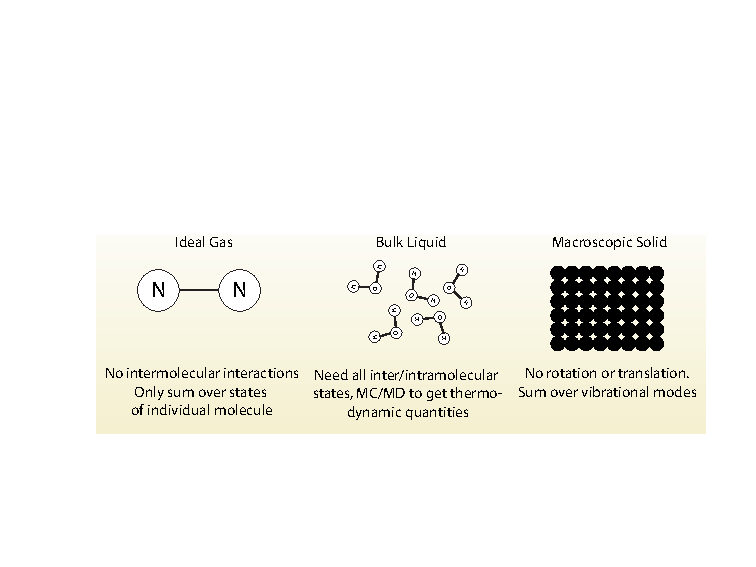
\includegraphics[width=.9\linewidth]{./Images/gls.pdf}
\end{center}

\subsubsection{Separability}
\label{sec:org333860d}

in principle need to sum over all the types of energy states (translational,
rotational, vibrational, \ldots{}) of every molecule.  Seemingly impossible task.
One simplification is if we can write energy as sum of energies of individual
elements (molecules) of system:
\begin{align}
  E_j&=\epsilon_j(1)+\epsilon_j(2) + ... + \epsilon_j(N) \\
  Q(N,V,T) &= \sum_j e^{-E_j\beta} \\
  &=\sum_je^{-(\epsilon_j(1)+\epsilon_j(2) + ... + \epsilon_j(N))\beta}
\end{align}
\emph{If} molecules/elements of system can be distinguished from each
        other (like atoms in a fixed lattice), expression can be factored:
  \begin{align}
    Q(N,V,T)&=\left ( \sum_j e^{-\epsilon_j(1)\beta}\right )\cdots \left ( \sum_j
      e^{-\epsilon_j(N)\beta}\right ) \\
  &= q(1)\cdots q(N) \\
  \text{Assuming all the elements are the same:}\\
  &= q^N
\end{align}
\emph{If not} distinguishable (like molecules in a liquid or gas, or
      electrons in a solid), problem is difficult, because identical
      arrangements of energy amongst elements should only be counted once.
      Approximate solution, good almost all the time:
\begin{equation}
  Q(N,V,T)=q^N/N!
\end{equation}
Sidebar: ``Correct'' factoring depends on whether individual elements
     are fermions or bosons, leads to funny things like superconductivity and
     superfluidity.

This \(q(V,T)\) is the \emph{molecular partition function}, and is calculated by
summing over the individual energy states of a single molecule (starting at \(E_0\)).

Further simplified by factoring into contributions from various (\(3N\)) molecular
degrees of freedom:
\begin{eqnarray}
  q(V,T)&=&\left(\sum_\mathrm{trans}
    e^{-e_\mathrm{trans}\beta}\right) \left(\sum_\mathrm{rot}
  e^{-e_\mathrm{rot}\beta}\right) \left( \sum_\mathrm{vib}
  e^{-e_\mathrm{vib}\beta} \right) \left( \sum_\mathrm{elec}
  e^{-e_\mathrm{elec}\beta}\right) \\
&=& q_\mathrm{trans}q_\mathrm{rot}q_\mathrm{vib}q_\mathrm{elec} \\
U & = & E_0 + U_\mathrm{trans}+U_\mathrm{rot}+U_\mathrm{vib}+U_\mathrm{elec}
\end{eqnarray}
Similarly for other thermodynamic quantities, for example,
\begin{equation}
  C_v=\left(\frac{\partial U}{\partial T}\right)_V = C_{v,\mathrm{trans}}+C_{v,\mathrm{rot}}+C_{v,\mathrm{vib}}+C_{v,\mathrm{elec}}
\end{equation}
Thermodynamic quantities are sums of contributions from indvidual degrees of
freedom.

Have to somehow \emph{model} these motions and have to use our quantum
mechanical results to parameterize the models.

\subsection{Ideal gas}
\label{sec:org5125250}
\subsubsection{Ideal gas of molecules}
\label{sec:orga43bc97}
Assume molecules are \emph{indistinguishable} and that internal energy is \emph{seperable}
\[  Q_{ig}(N,V,T) = \frac{(q_\mathrm{trans}q_\mathrm{rot}q_\mathrm{vib}q_\mathrm{elec})^N}{N!} \]
\[ F(N,V,T) = F_\mathrm{trans}+ F_\mathrm{rot} + F_\mathrm{vib}+F_\mathrm{elec}\]
for any thermodynamic function \(F\).
\subsubsection{Electronic partition functions \(\rightarrow\) spin multiplicity}
\label{sec:org4e590dc}
Governed by Fermi-Dirac distribution. Electronic degeneracy at normal \emph{T}.
\subsubsection{Vibrational thermodynamics: harmonic oscillator}
\label{sec:orgc175e42}
Energy spectrum above ZPE given
\begin{equation}
  E_v=hv\nu,\qquad v=0,1,2,...
\end{equation}
Define characteristic temperature \(\Theta =h \nu/k_B\).
\begin{eqnarray}
q(T) & = &\sum_{v=0}^\infty e^{-v(\Theta/T)} \\
 & = & \frac{1}{1-e^{-\Theta/T}}
\end{eqnarray}
(geometric series). Partition function increasing function of \emph{T}.  Look at limits.

\noindent Internal energy:
\begin{eqnarray}
  U(T) &=&-\frac{\partial \ln q}{\partial \beta}\\
   & = & \frac{\epsilon_0}{e^{\epsilon_0\beta}-1}
\end{eqnarray}
Need vibrational spectrum to get these contributions.

\emph{Results only as good as H-O model!} For low frequency modes, errors can be substantial, esp for entropy.  Can apply more sophisticated models.

\subsubsection{Rotational thermodynamics: rigid  rotor}
\label{sec:org1148d4e}
Characteristic temperature \(\Theta_\mathrm{rot} = \hbar^2/2 I k_B\).  Moment of intertia \emph{I} only depends on shape or molecule---geometry optimzation. 

``High'' T \(q_\mathrm{rot}(T) \approx \sigma \Theta_\mathrm{rot}/T\), most often true
\subsubsection{Translational states: particle-in-a-box}
\label{sec:orged06629}
\[
  E_n=\frac{n^2\pi^2\hbar^2}{2 m L^2} = \epsilon_0n^2,\qquad n=1,2,3,\ldots
\]
\(\Theta_\mathrm{trans} = \epsilon_0/k_B\) is typically tiny, allows partition function sum to be approximated by integral:
\begin{eqnarray*}
q_\mathrm{trans,1D} \approx \int_0^\infty e^{-x^2\beta\epsilon_0}dx =
             L/\Lambda \\
             \Lambda = \frac{h}{\sqrt{2\pi m k_B T}} \qquad
             \mathrm{thermal\ wavelength} \\
             q_\mathrm{trans,3D} = V/\Lambda^3
           \end{eqnarray*}

Thermal wavelength \(\Lambda\) depends only a molecule mass and is of the order the box
dimensions at which quantization is evident.  Typically a tiny number
(eg \SI{1.7e-11}{m} for Ar in a \SI{1}{\liter} volume at \SI{298}{K}.
\(q_\mathrm{trans}\) is thus enormous: lots of translational freedom.  \(q\) depends on volume, introduces volume/concentration/pressure dependence into thermo functions.  Conventional to define a \emph{standard state} \(V^\circ\) volume, or corresponding pressure.


\begin{table}
\begin{center}
    \caption{\large{Statistical Thermodynamics of an Ideal Gas}}
   \begin{description}
    \item[\underline{Translational DOFs}] {3-D particle in a box model}

$\displaystyle \theta_\mathrm{trans}= \frac{\pi^2\hbar^2}{2 m
  L^2 k_B}$,
$\displaystyle \Lambda=h\left( \frac{\beta}{2\pi m}\right )^{1/2}$

For $ T >> \Theta_\mathrm{trans}$, $\Lambda << L$, $\displaystyle
q_\mathrm{trans}=V/\Lambda^3$ (essentially always true)

\begin{tabular}{ccc}
$\displaystyle U_\mathrm{trans}=\frac{3}{2}RT$ & $\displaystyle C_\mathrm{v,trans} =
\frac{3}{2}R $ & $\displaystyle S^\circ_\mathrm{trans}=R \ln \left (
  \frac{e^{5/2}V^\circ}{N^\circ \Lambda^3}\right ) = R \ln \left (
  \frac{e^{5/2}k_BT}{P^\circ \Lambda^3}\right ) $ \\
\end{tabular}

  \item[\underline{Rotational DOFs}] {Rigid rotor model}
\begin{description}
\item[Linear molecule]{}
$\theta_\mathrm{rot} =hcB/k_B$

\begin{equation*}
q_\mathrm{rot}=\frac{1}{\sigma}\sum_{l=0}^\infty (2l+1)e^{-l(l+1)\theta_\mathrm{rot}/T},
\approx \frac{1}{\sigma}\frac{T}{\theta_\mathrm{rot}},\ \ T>>\theta_\mathrm{rot}\ \ \ \sigma = \left \{
        \begin{array}{rl}
          1, & \text{unsymmetric} \\
          2, & \text{symmetric}
        \end{array} \right .
\end{equation*}
\begin{tabular}{ccc}
$\displaystyle U_\mathrm{rot}=RT$ & $\displaystyle C_\mathrm{v,rot} =
R $ & $\displaystyle S^\circ_\mathrm{rot}=R (1-\ln(\sigma\theta_\mathrm{rot}/T)) $ \\
\end{tabular}


\item[Non-linear molecule]{} $\theta_{\mathrm{rot},\alpha}=hcB_\alpha/k_B$
\begin{equation*}
q_\mathrm{rot} 
\approx \frac{1}{\sigma}\left ( \frac{\pi
    T^3}{\theta_{\mathrm{rot},\alpha}\theta_{\mathrm{rot},\beta}\theta_{\mathrm{rot},\gamma}}
  \right )^{1/2},\ \ T>>\theta_{\mathrm{rot},\alpha,\beta,\gamma}\ \ \ \sigma =
  \text{rotational symmetry number}
\end{equation*}
\begin{tabular}{ccc}
$\displaystyle U_\mathrm{rot}=\frac{3}{2}RT$ & $\displaystyle C_\mathrm{v,rot} = \frac{3}{2}
R $ & $\displaystyle S^\circ_\mathrm{rot}=\frac{R}{2}
\left ( 3-\ln\frac{\sigma\theta_{\mathrm{rot},\alpha}\theta_{\mathrm{rot},\beta}\theta_{\mathrm{rot},\gamma}}{\pi
  T^3} \right ) $ \\
\end{tabular}

\end{description}

\item[\underline{Vibrational DOFs}] {Harmonic oscillator model}
\begin{description}
\item[Single harmonic mode] {$\theta_\mathrm{vib}=h\nu/k_B $}
  \begin{equation*}
    q_\mathrm{vib}=\frac{1}{1-e^{-\theta_\mathrm{vib}/T}} \approx
      \frac{T}{\theta_\mathrm{vib}}, \ \ \ T>>\theta_\mathrm{vib}
  \end{equation*}

\begin{tabular}{ccc}
$ U_\mathrm{vib}= $ & $  C_\mathrm{v,vib} = $ & $S^\circ_{\mathrm{vib},i}=$ \\
$\displaystyle
R\frac{\theta_\mathrm{vib}}{e^{\theta_\mathrm{vib}/T}-1}$ &
$\displaystyle R\left (
  \frac{\theta_\mathrm{vib}}{T}\frac{e^{\theta_\mathrm{vib}/2T}}{e^{\theta_\mathrm{vib}/T}-1}
\right )^2 $ & $\displaystyle R \left ( \frac{\theta_\mathrm{vib}/T}{e^{\theta_\mathrm{vib}/T}-1}
-\ln(1-e^{-\theta_\mathrm{vib}/T})\right ) $ \\
\end{tabular}

\item[Multiple harmonic modes] {$\theta_{\mathrm{vib},i}=h\nu_i/k_B $}

  \begin{equation*}
    q_\mathrm{vib}=\prod_i\frac{1}{1-e^{-\theta_{\mathrm{vib},i}/T}} 
  \end{equation*}

\begin{tabular}{ccc}
$ U_\mathrm{vib}= $ & $  C_\mathrm{v,vib} = $ & $S^\circ_{\mathrm{vib},i}=$ \\
$\displaystyle
R\sum_i\frac{\theta_{\mathrm{vib},i}}{e^{\theta_{\mathrm{vib},i}/T}-1}$ &
$\displaystyle R \sum_i \left (
  \frac{\theta_{\mathrm{vib},i}}{T}\frac{e^{\theta_{\mathrm{vib},i}/2T}}{e^{\theta_{\mathrm{vib},i}/T}-1}
\right )^2 $ & $\displaystyle R \left ( \frac{\theta_{\mathrm{vib},i}/T}{e^{\theta_{\mathrm{vib},i}/T}-1}
-\ln(1-e^{-\theta_{\mathrm{vib},i}/T})\right ) $ \\
\end{tabular}

\end{description}
\item[\underline{Electronic DOFs}] {}
$q_\mathrm{elec} = \text{spin multiplicity}$


\end{description}
\end{center}
\end{table}

\begin{table}[htbp]
\caption{Contributions to ideal gas thermodynamics}
\centering
\begin{tabular}{lllll}
\hline
 & Characteristic & Characteristic & States @ RT & \\
 & Energy (cm\(^{\text{-1}}\)) & Temperature (K) &  & \\
\hline
translational & \(\hbar^2/2 m L^2 \approx 10^{-21}\) & \(10^{-21}\) & \(10^{30}\) & classical limit\\
 &  &  &  & \\
rotational & \(\approx 1\) & \(\approx 1\) & 100's & semi-classical\\
 &  &  &  & \\
vibrational & \(\approx 1000\) & \(\approx 1000\) & 1 & non-classical\\
 &  &  &  & \\
electronic & \(\approx 10,000\) & \(\approx 10,000\) & 1 & non-classical\\
\hline
\end{tabular}
\end{table}

\begin{table}
   \caption{Ethane thermodynamics}
\begin{tabular}{cc}
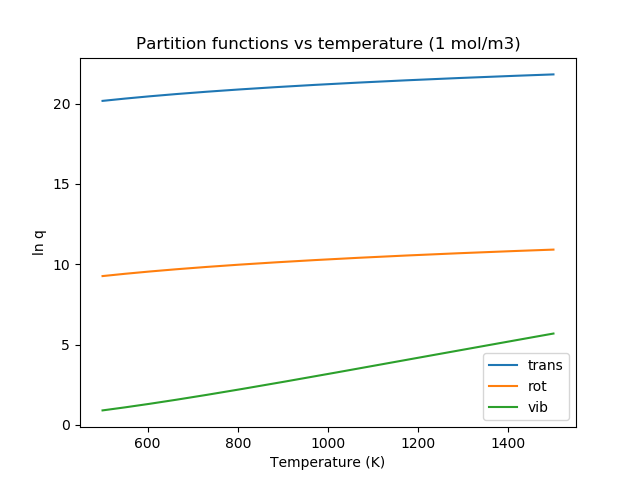
\includegraphics[scale=0.5]{./Images/ethane-partition.png} & 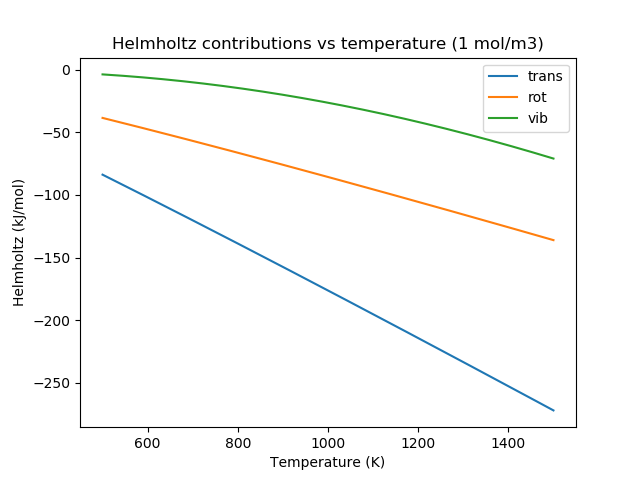
\includegraphics[scale=0.5]{./Images/ethane-helmholtz.png} \\
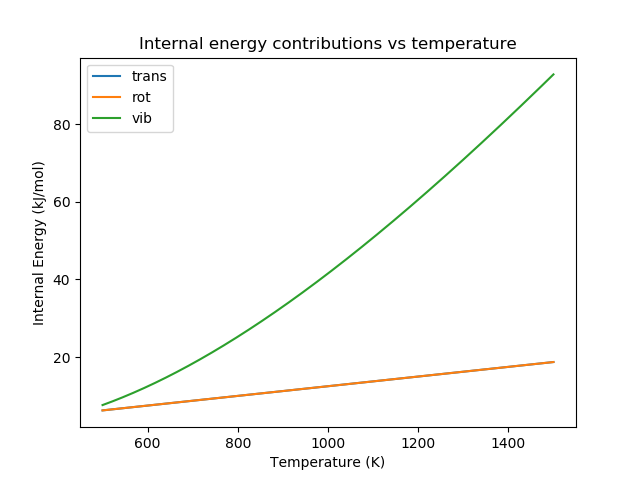
\includegraphics[scale=0.5]{./Images/ethane-energy.png} & 
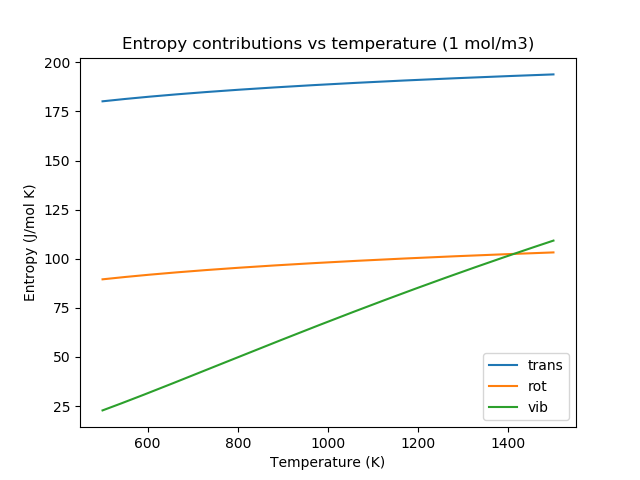
\includegraphics[scale=0.5]{./Images/ethane-entropy.png}
\end{tabular}
\end{table}

\subsection{Chemical reactions and equilibria}
\label{sec:orgc005879}
\subsubsection{Chemical reaction}
\label{sec:org860d164}
\begin{enumerate}
\item General chemical reaction \(\sum_i \nu_i A_i = 0\), \(\nu_i\) stoichiometric coefficients
\item Thermodynamic change \(\Delta W^\circ(T) = \sum_i \nu_i W^\circ_i(T)\), where \(W = A, U, S, G, \ldots\)
\item ``Standard state'' derives from concentration dependence of entropy
\item ``Standard state'' corresponds to some standard choice, \((N/V)^\circ = c^\circ\), e.g. \SI{1}{mol/l} (T-independent), or \((N/V)^\circ = P^\circ/RT\), e.g. \SI{1}{bar} (T-dependent)
\item Permits functions to be easily computed at other concentrations, e.g.
\begin{displaymath}
A(T,N/V)  = A^\circ(T) + k T \ln\left ( (N/V)/(N/V)^\circ \right ) =A^\circ(T) + k T \ln \left ( c/c^\circ \right )
\end{displaymath}
\item Example: ethane dehydrogenation, \ce{C2H6 -> C2H4 + H2}, 1 bar standard state
\item Reaction entropy captures contributions of all degrees of freedom
\item Reaction energy (internal, Helmholtz, \ldots{}) must \emph{also} capture difference
in \SI{0}{K} electronic energy
  \begin{displaymath}
\Delta U^\circ (T) = U^\circ_\mathrm{B}(T)-U^\circ_\mathrm{A}(T)+\Delta E(0)
   \end{displaymath}
\end{enumerate}
\begin{table}
   \caption{Ethane to ethylene plus hydrogen standard state (1 bar) thermodynamcs}
\begin{tabular}{cc}
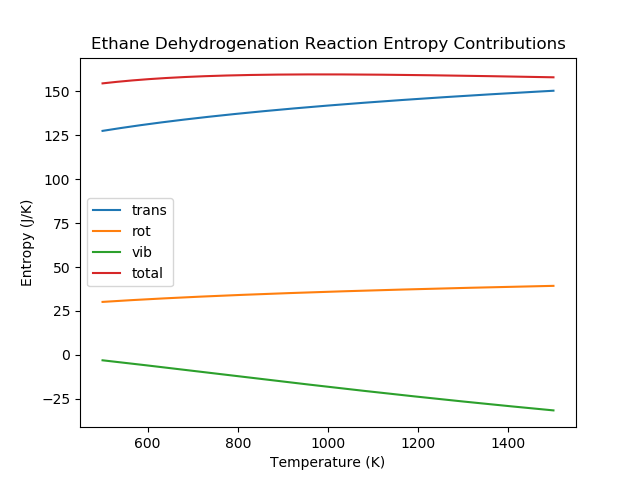
\includegraphics[scale=0.5]{./Images/dehydro-entropy.png} & 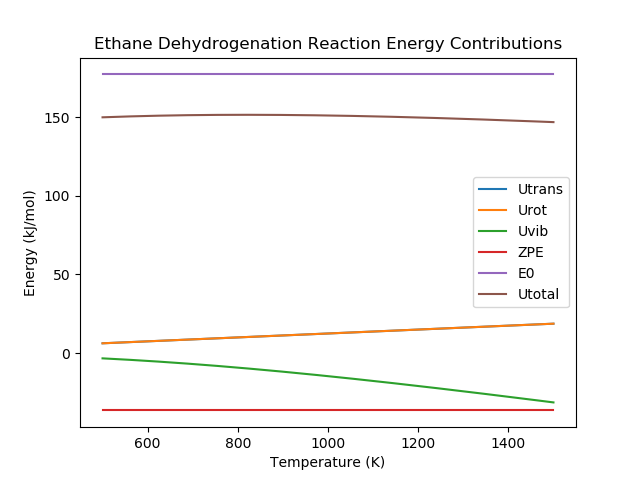
\includegraphics[scale=0.5]{./Images/dehydro-energy.png} \\ \includegraphics[scale=0.5]{./Images/dehydro.png} & \includegraphics[scale=0.5]{./Images/dehydroG.png} \\
\includegraphics[scale=0.5]{./Images/equilibrium.png} 
\end{tabular}
\end{table}

\subsubsection{Chemical equilibrium}
\label{sec:org78afc12}
\begin{enumerate}
\item At chemical equilbrium, total free energy minimized with respect to reaction advancement \(\xi\)
\[G(T,\xi) = \xi  (\Delta G^\circ + k T \sum_i \nu_i \ln P_i/P^\circ) \]
\item Equilibrium condition---equate chemical potentials
  \begin{eqnarray*}
 \mu_A(N,V,T) & = & \mu_B(N,V,T) \\
 E_A(0) - k T \ln (q_A/N_A) & = & E_B(0) - k T \ln (q_B/N_B) \\
\frac{N_B}{N_A} =  \frac{N_B/V}{N_A/V} & = &\frac{q_B(T,V)/V}{q_A(T,V)/V} e^{-\Delta E(0)/kT}
  \end{eqnarray*}
\item \(q/V = 1/\Lambda^3\) has units of number/volume, or concentration
\item Equilibrium constant---convert units to some standard concentration \(c^\circ\) or pressure \(P^\circ\)
 \begin{eqnarray*}
  q_A^\circ(T) & = & (q_A(T,V)/V) (1/c^\circ) \\
  q_A^\circ(T) & = & (q_A(T,V)/V)(RT/P^\circ) \\ 
K_{eq}(T) & = &\frac{q_B^\circ(T)}{q_A^\circ(T)} e^{-\Delta E(0)/kT} = e^{-\Delta G^\circ(T)/kT} 
 \end{eqnarray*}
\end{enumerate}

\subsection{Reaction rates}
\label{sec:orgf867146}
Rate: number per unit time per unit something (volume, area, \ldots{}).  Reactions hypothesized to occur through sequence of elementary steps.

For example, ozone decomposition, rate second-order at high \(P_{\ce{O2}}\), first-order at low \(P_{\ce{O2}}\)
\begin{center}
\begin{tabular}{l}
\ce{2 O3 -> 3 O2}\\
\hline
\ce{O3 ->[k_1] O2 + O}\\
\ce{O2 + O ->[k_-1] O3}\\
\ce{O + O3 ->[k_2] 2 O2}\\
\end{tabular}
\end{center}


See two compute rates of individual steps.

\subsubsection{Transition state theory (TST)}
\label{sec:org8ec1aff}
\begin{enumerate}
\item Assumptions
\begin{enumerate}
\item Existence of reaction coordinate (PES)
\item Existence of dividing surface
\item Equilibrium between reactants and ``transition state''
\item Harmonic approximation for transition state
\end{enumerate}
\item rate proportional to concentration of ``activated complex'' over reactants times crossing frequency
\begin{eqnarray*}
   r & = & k C_AC_B \\
     & = & k^\ddagger C_{AB}^\ddagger \\
     & = & \nu^\ddagger K^\ddagger C_A C_ B \\
     & = & \nu^\ddagger \frac{k_BT}{h\nu^\ddagger}\bar{K}^\ddagger(T) C_A C_B \\
     & = & \frac{k_B T}{h} \frac{q^\ddagger(T)}{q_A(T) q_B(T)}  e^{-{\Delta E(0)/k_BT}} C_A C_B
\end{eqnarray*}
\item application to two molecules - vinyl alcohol to acetaldehyde
\item microscopic reversibility
\item equilibrium requirement \(K_{eq}(T) = k_f(T)/k_r(T)\)
\end{enumerate}
\begin{center}
\includegraphics[width=0.6\textwidth]{./Images/PES2.png}
\end{center}
\subsubsection{Thermodynamic connection}
\label{sec:orgbd7e6d5}
\begin{enumerate}
\item Relate activated complex equilibrium constant to activation free energy
\[ \(\bar{K}^\ddagger(T) = e^{-\Delta G^{\circ \ddagger}(T)/kT} = e^{-\Delta H^{\circ \ddagger}(T)/k_BT}e^{\Delta S^{\circ \ddagger}(T)/k_B} \]
\item Compare to Arrhenius expression 
\[E_a = \Delta H^{\circ \ddagger}(T) + kT, A = \frac{k_B T}{h}e^1e^{\Delta S^{\circ \ddagger}(T)/k_B}\]
\end{enumerate}

\begin{table}
   \caption{Vinyl alcohol to acetaldehyde}
\begin{tabular}{cc}
\includegraphics[scale=0.5]{./Images/kTh.png} & \includegraphics[scale=0.5]{./Images/qratio.png} \\ \includegraphics[scale=0.5]{./Images/expEa.png} & \includegraphics[scale=0.5]{./Images/halflife.png} \\
\includegraphics[scale=0.5]{./Images/arrhenius.png} & 
\includegraphics[scale=0.3]{./Images/Path.png} 
\end{tabular}
\end{table}

\newpage

\section{Plane waves and core potentials}
\label{sec:orgabccabf}
\subsection{Periodic boundary conditions}
\label{sec:orge42c65e}
Free particle moving in one dimension
\[\phi_G(x) = e^{i G x} \]
\emph{G} can take any value. Eigenfunction of momentum and kinetic energy operators.  In particular,
\[E_G = \frac{\hbar^2}{2m}G^2\]

Suppose we impose \emph{periodic boundary conditions}, so that \(\phi_G(x) = \phi_G(x+na), n=\pm 1, \ldots\).  \emph{a} is a \uline{lattice vector}.
\[e^{i G x} = e^{i G (x + a)} \rightarrow e^{i G a} = 1\]
Places constraints on \emph{G}:
\[ G = \frac{2\pi}{a} n, n = \pm 1, \ldots\]
\(2\pi/a\) is a \uline{reciprocal lattice vector}.

Normalized on domain \emph{a},
\[\phi_G(x) = \frac{1}{\sqrt{a}}e^{i G x}\]

Properties of these \uline{plane wave} functions:
\begin{enumerate}
\item Periodic, \(\lambda_G = a/n\)
\item Orthonormal, \(\langle \phi_G | \phi_{G^\prime}\rangle = \delta_{G,G^\prime}\)
\item Definite kinetic energy
\item Complete
\begin{eqnarray}
  \psi(x) &=& \sum_G \phi_G(x) \langle \phi_G | \psi \rangle \\
          & = & \sum_G \phi_G(x) \psi(G)
\end{eqnarray}
\end{enumerate}

\(\psi(G)\) is Fourier transform of \(\psi(x)\).  Both contain exactly the same information. Can take advantage of Fourier transform machinery to transform between two representations.  For general function \(\psi(x)\), represent on some grid of size \emph{N}.  Size of grid determined by maximum frequency/minimum wavelength included.  \(N\log(N)\) operations to transform back and forth.

Integrals can be evaluated in either \emph{x} or \emph{G} space:
\begin{eqnarray}
I & = & \int_a A^*(x) B(x) d x \\
  & = & \sum_{G,G^\prime} A^*(G) B(G) \int e^{-iGx}e^{iG^\prime x} dx \\
  & = & \sum_{G,G^\prime} A^*(G) B(G) \delta_{G,G^\prime} \\
  & = & a \sum_G A^*(G) B(G)
\end{eqnarray}
Can leverage to simplify solving any problems that are periodic.

\subsection{Hydrogen atom in a box}
\label{sec:org59ceca8}
Suppose we place an atom at some point \emph{R} in each box.  In principle, can  represent solutions as linear combinations of plane waves.  Plane waves become basis functions. 

Does where we put the atom matter to the answer? No. Alway related by \uline{structure factor}.

In principle, would have to let \emph{G} run to infinity to have complete basis. In practice, would have to cut off at some point, defined by
\[ \frac{\hbar^2}{2 m_e} G^2 < \frac{\hbar^2}{2 m_e} G_\text{cut}^2 = E_\text{cutoff} \]
Sets minimum wavelength retained in basis, and thus size of basis. For fixed \(E_\text{cutoff}\), larger \emph{a} implies larger basis.  Basis size has to be a whole number, so changes discontinuously with \(E_\text{cutoff}\).

Recall our basic equation
\begin{equation}
\left \{ \hat{h} +v_{\text{Coulomb}}[\rho] + v_\text{exchange}[\psi_{i}] + v_\text{correlation}[\psi_{i}]\right\}\psi_i(\mathbf{r}) =\epsilon_i \psi_i(\mathbf{r})
\end{equation} 
Contains kinetic and potential energy terms.

\uline{Kinetic energy} is diagonal in plane wave basis\ldots{}easy!
\[ \langle \phi_G | -\frac{1}{2}\frac{d^2}{dx^2} | \phi_{G^\prime} \rangle = \frac{1}{2}G^2 \delta_{G,G^\prime} \]

\uline{Potential energy terms} can take advantage of Fourier transforms.
\begin{eqnarray}
v(x) & = & \sum_{G^{''}} v(G'') e^{i G'' x}  \\
\langle \phi_G | v(x) | \phi_{G'}\rangle & = & \sum_{G^{''}} v(G'') \langle \phi_G | \phi_{G''} |  \phi_{G'} \rangle \\
 & = & v(G'-G) 
\end{eqnarray}
How many Fourier components to include in the sums? Turns out for a basis of dimension \emph{m} you need \emph{2m} components to specify the potential exactly, but you can generally get away with smaller. The cost and accuracy of the calculation scale with this choice.

Solutions given by \(\psi_i(x) = \sum_G c_i(G) \phi_G(x)\).

One key thing we would need to evaluate potentials is \uline{electron density}, \(\rho(x)\).  Let \(f_i\) be occupancy of each orbital.
\begin{eqnarray}
 \rho(x) & = & \sum_i f_i |\psi_i(x)|^2 \\
         & = & \frac{1}{a}\sum_i f_i \sum_{G,G'} c_i^*(G)c_i(G') e^{i(G-G')x} \\
	 & = & \sum_{-2 G_\mathrm{max}}^{2 G_\mathrm{max}} n(G) e^{i G x} 
\end{eqnarray}
Electron density exactly represented in plane wave basis with cutoff four times that of the basis set cutoff.

\subsection{Three-dimensional periodicity}
\label{sec:orgcfefb46}
Same ideas generalize to three dimensional periodicity.

\uline{Lattice constants} of periodic cell become three vectors, \(\bm{a}_1\), \(\bm{a}_2\), \(\bm{a}_3\).  As we'll discuss a little bit later, these vectors will be from one of the Bravais lattices.  Every point \bm{R} is equivalent to any other point \(\bm{R}'=\bm{R} + n_1 \bm{a}_1+ n_2 \bm{a}_2+ n_3 \bm{a}_3\).

Periodic box matrix \(\bm{h} = [\bm{a}_1, \bm{a}_2,\bm{a}_3]\).  Periodic box volume \(\Omega = \text{det} \bm{h}\).

\uline{Reciprocal lattice} defined such that \(\bm{b}_i\cdot\bm{a}_j = 2 \pi \delta_{ij}\).  Given by
\[2\pi(\bm{h}^t)^{-1} = [\bm{b}_1,\bm{b}_2,\bm{b}_3]\]

\uline{Reciprocal lattice vectors} become \(\bm{G} = i \bm{b}_1 + j \bm{b}_2 + k \bm{b}_3\).  Basis functions become \(\phi(\bm{r}) = \frac{1}{\Omega}e^{i \bm{G}\cdot\bm{r}}\).

Locations of atoms \(\bm{R}_\alpha\) within this periodic cell can be specified in Cartesians or as fractional coordinates of the lattice vectors.  Related by \(\bm{R}_\alpha = \bm{h}\bm{f}\).

In general, can use this periodic representation to describe atoms, molecules, whatever.  If we want to describe isolated things, box dimensions must be large enough to avoid artificial interactions between periodic images. 

In particular, Coulomb potentials decay like \(1/r\) and are thus long-ranged.  Have to use special tricks (Ewald sums) to evaluate these sums, and have to carefully group electrostatic terms to avoid non-convergent sums.

Key limitations:
\begin{enumerate}
\item Periodic cell must be charge-neutral.  The electrostatic energy of an infinite, charged system diverges.
\item Supercell must not have a net electric field.
\item The absolute electrostatic potential is not well-defined (there is no ``vacuum'' to reference the energy of an electron to).
\end{enumerate}
These limitations can be overcome to some extent by applying artificial backgrounds.
\subsection{Gaussian vs. Vasp}
\label{sec:org851d645}

\subsection{Vasp POSCAR}
\label{sec:orgfc6264a}

\subsection{Vasp INCAR}
\label{sec:org44fac5c}

\subsection{Core electron treatment}
\label{sec:orgc3dcb36}

\subsubsection{OPW}
\label{sec:orga6b5522}

\subsubsection{PP}
\label{sec:orge988848}

\subsubsection{PAW}
\label{sec:org153ef90}

\subsection{Comparing energies between calculations}
\label{sec:org59e514a}

\subsection{Wavefunctions and charge densities}
\label{sec:orge18b762}

\subsection{Exploring potential energy surfaces}
\label{sec:org97f5110}
\newpage
\section{Periodic electronic structure}
\label{sec:org7354487}
\subsection{Isolated vs. periodic systems}
\label{sec:orgf98bc35}
\subsection{Bloch's theorem and qualitative band structure}
\label{sec:org7e1806e}
\subsection{Band folding}
\label{sec:org68f18be}
\subsection{Multi-dimensional periodicity}
\label{sec:orgd2421c9}
\subsection{Density of statues}
\label{sec:orge14d72c}
\subsection{Bravais lattices}
\label{sec:orge0c7d8b}
\subsection{Quantitative supercell calculations}
\label{sec:org1f63985}
\subsection{Brillouin zone integration}
\label{sec:orgdf29289}
\subsubsection{k-point sampling}
\label{sec:org26305ad}
\subsubsection{Fermi smearing}
\label{sec:org03b491b}
\newpage
\section{Practical supercell calculations}
\label{sec:org0b1280f}
\newpage
\section{Surfaces}
\label{sec:org709abcc}
\subsection{Surface planes}
\label{sec:orga9c437a}
\subsection{Slab models}
\label{sec:org015cd3d}
\subsection{Surface energy}
\label{sec:org7b3503f}
\subsection{Surface potentials and Fermi energies}
\label{sec:orgc543008}
\subsection{Surface adsorption}
\label{sec:org6c3e063}
\subsection{Coverage-dependent adsorption}
\label{sec:orga015e09}
\subsection{Reaction barriers}
\label{sec:org7a5047d}

\newpage
\section{Implicit solvation}
\label{sec:org82fa159}
\section{Density functional theory}
\label{sec:org612d008}
\subsection{Electron density \(\rho\) as fundamental quantity}
\label{sec:org901cc5d}
\subsection{Thomas-Fermi-Dirac model}
\label{sec:orgdd9a30a}
\subsection{Hartree-Fock-Slater model}
\label{sec:org3a28140}
\subsection{Hohenberg-Kohn theorems}
\label{sec:orgd774f49}
\subsection{Kohn-Sham construction}
\label{sec:orgff6e8ac}
\subsection{Exchange-correlation functionals}
\label{sec:org6c0b47e}
So Kohn et al. showed that the DFT approach is theoretically well-grounded and
provided one way to practically apply it. Promise is that if we can find an
approximation to the (unknown) true \(v_\text{xc}\) with the right balance of simplicity
and accuracy, we will have one sweet theory. Has to incorporate both exchange,
like Slater tried to do, and correlation.

How to proceed? Lots of approaches, and jargon here is at least as bad as in
wavefunction-based methods. Perdew 2006 describes the ``Jacob's ladder'' of
approximations:
\subsubsection{LDA}
\label{sec:org27aa33e}
One well-defined limit is the homogeneous electron gas, and this is the usual
starting point for modern approximate DFT methods. Assume exchange and
correlation potentials at any given point depend only on the value of \(\rho\) there
(or spin-up and spin-down \(\rho\), if spin-polarized). We know from Slater and
Dirac's work what the exchange potential is for this system.

It is possible to determine numerically the correlation energy for a given
density from quantum Monte Carlo calculations. Ceperley and Alder (PRL 1980,
45, 566) did this to very high accuracy, and others (Vosko, Wilk, and Nusair,
``VWN'', and Perdew and Wang, ``PW'') fit these numerical results to analytical
models in \(\rho\). This combination of local exchange and correlation defines the LDA
model.

LDA offers modest improvement over HFS for molecules. ``Homogeneous''
approximation pretty severe for an atom or molecule. Nonetheless, works
surprisingly well for structures and charge distributions, but has problems in
calculating accurate bond energies, typically overbinding. Also tends to
underestimate the HOMO-LUMO gap in molecules and analogous band gap in solids.

\subsubsection{GGA}
\label{sec:org1f30b81}

\subsubsection{Meta-GGA}
\label{sec:org707839f}

\subsubsection{Hyper GGA and hybrid functionals}
\label{sec:org86ac945}

\begin{itemize}
\item ``Screened'' exchange
\label{sec:org80bcc18}
\end{itemize}

\subsubsection{Beyond hyper GGA}
\label{sec:org6ca7767}

\subsection{Implementations}
\label{sec:org96cf2e8}

\subsection{Performance}
\label{sec:orge6c767a}
\newpage
\newpage
\section{Electron correlation methods}
\label{sec:orgcda3677}
\newpage
\end{document}